\chapter{Additional Model Results}
\label{appn:modelresults}

\section{Verification Plots for Poor Performing Models}

\subsection{Storm Maximum Intensity First Points Only}

\begin{figure}[h]
    \centering
    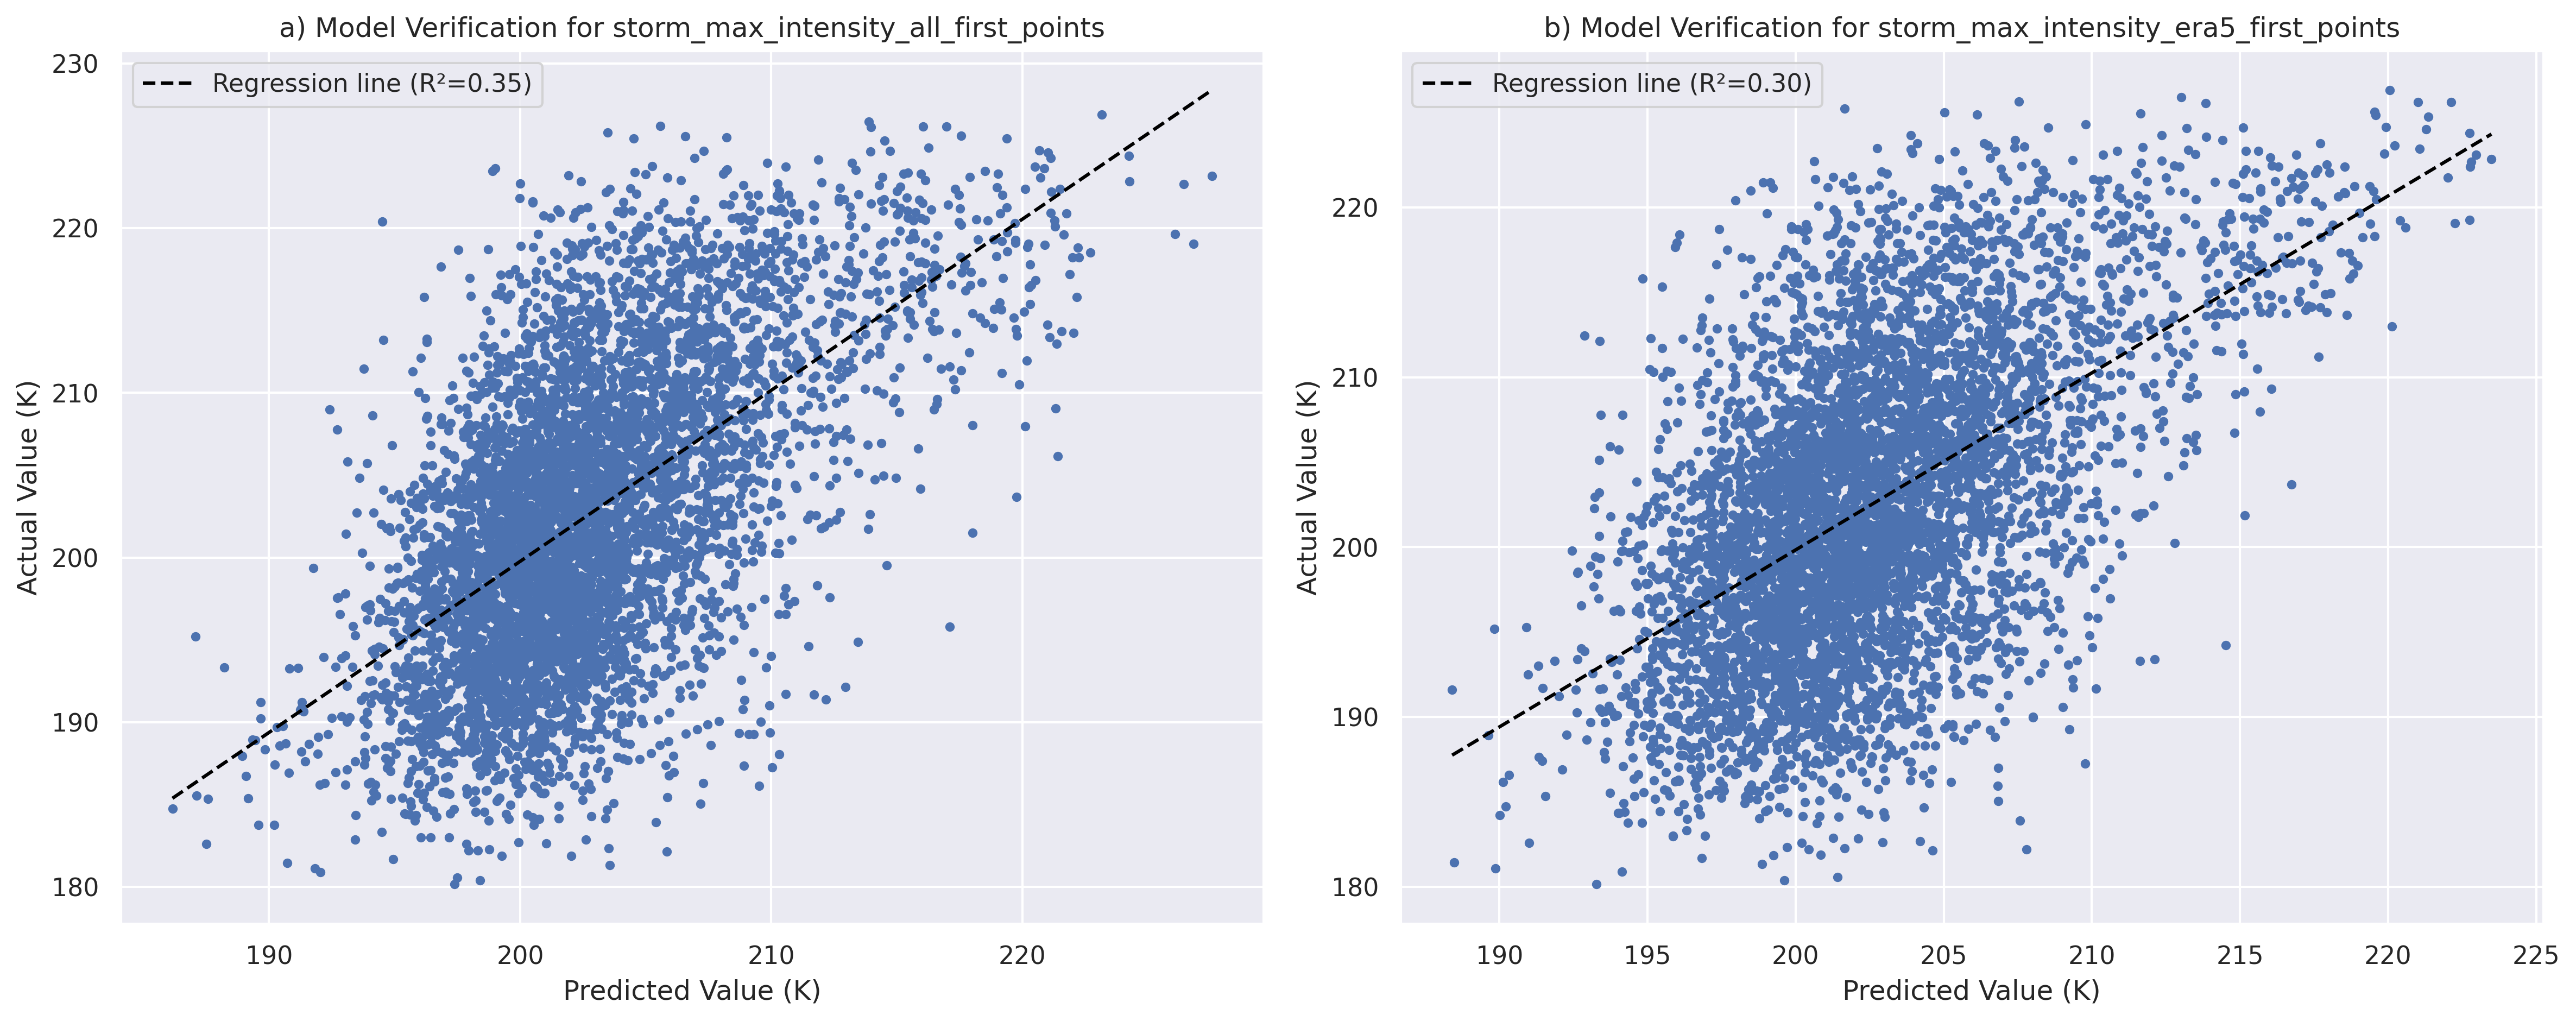
\includegraphics[width=\textwidth]{../figures/generated/experiments/storm_max_intensity_first_points/storm_max_intensity_first_points_summary.png}
    \caption{Comparison of performance and top features for storm maximum intensity (First Points Only).}
    \label{fig:storm_max_intensity_first_points_summary}
\end{figure}

\subsubsection{Storm Direction First Points Only}

\begin{figure}[h]
    \centering
    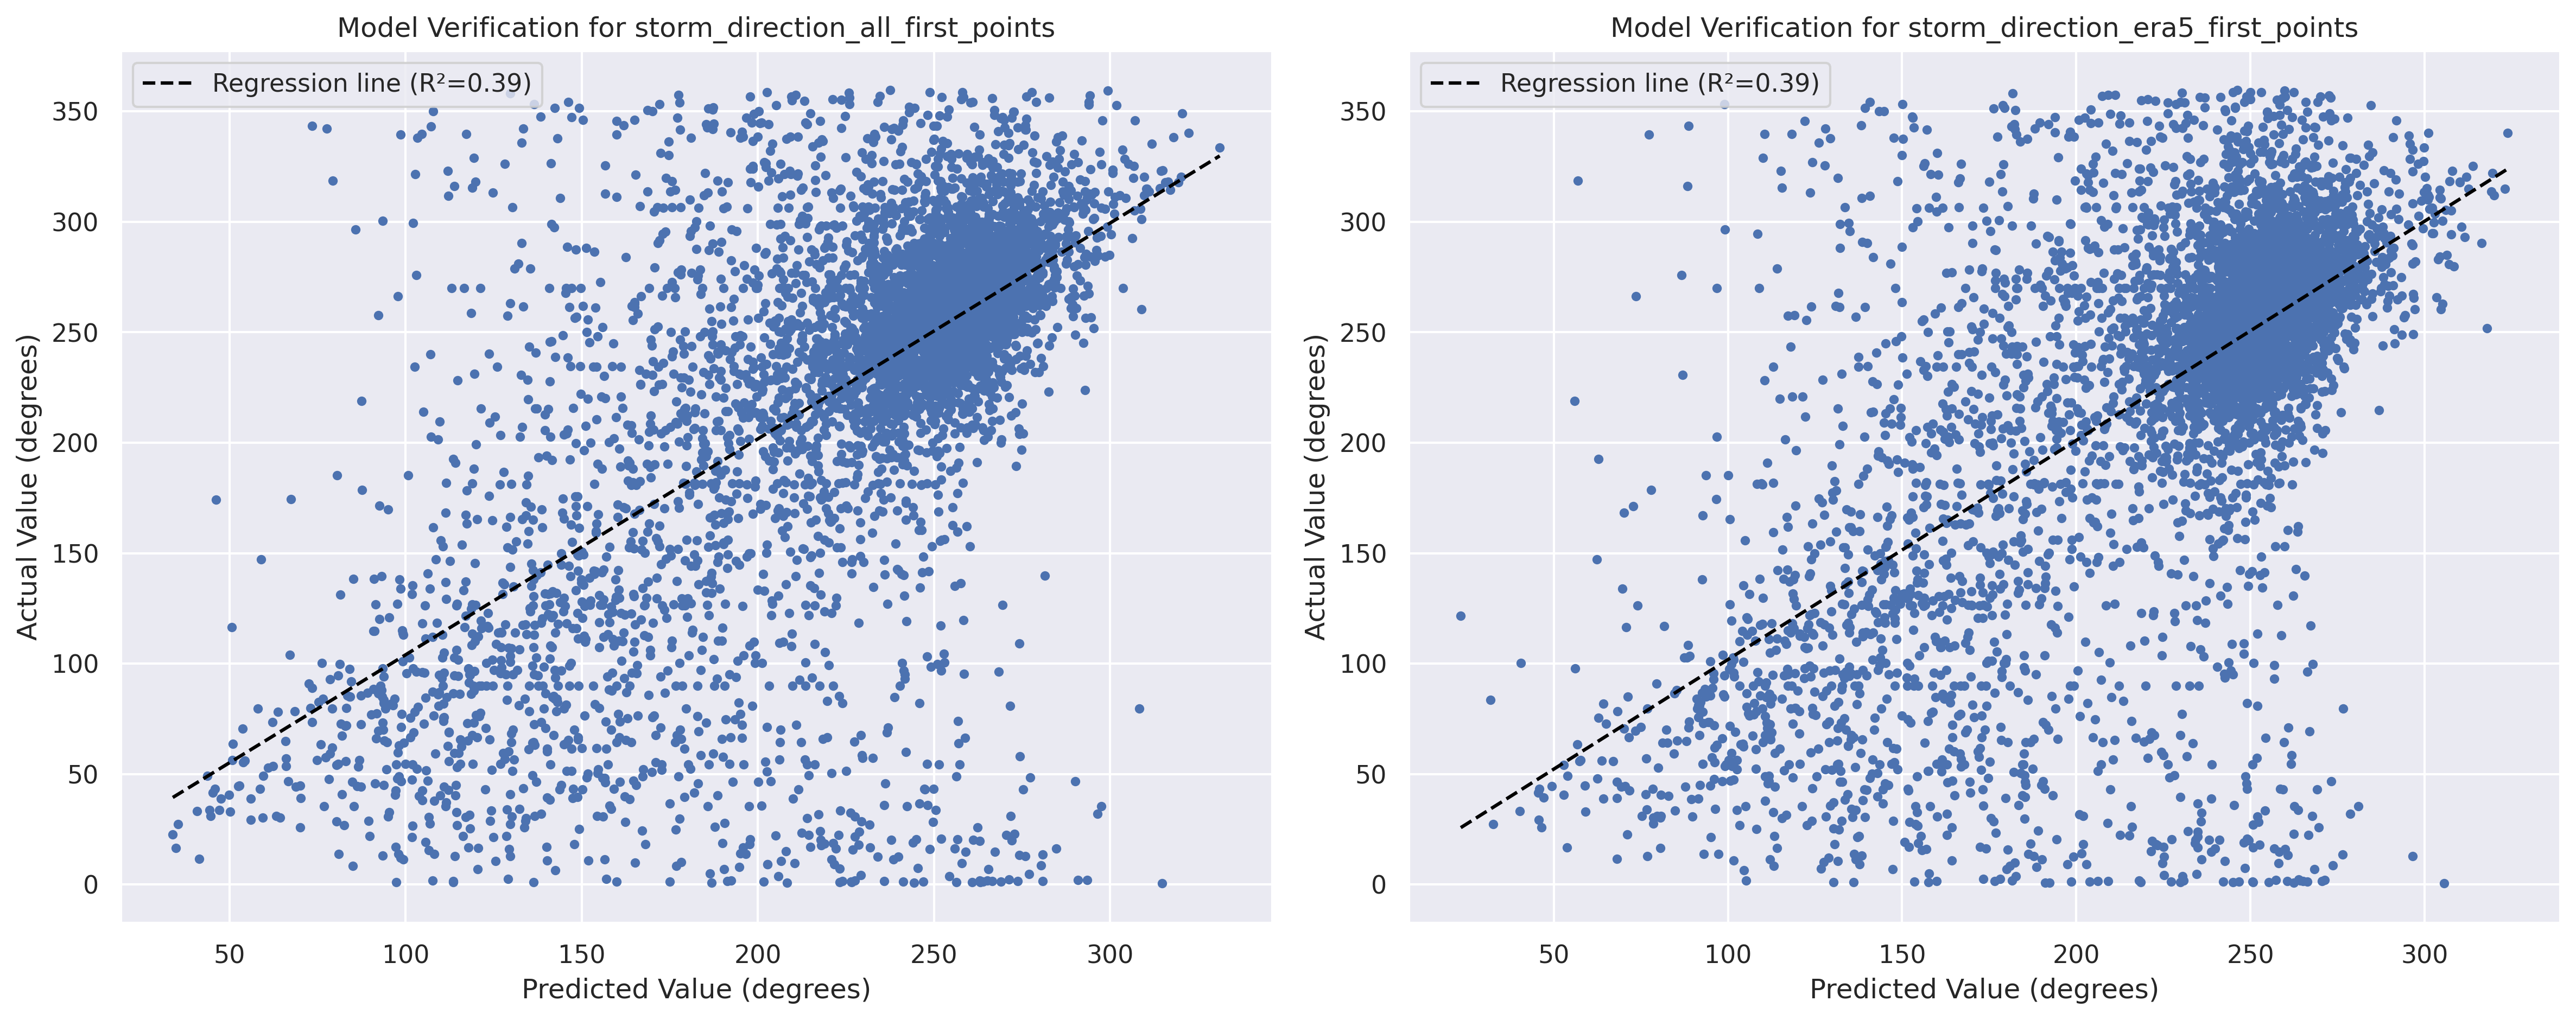
\includegraphics[width=\textwidth]{../figures/generated/experiments/storm_direction_first_points/storm_direction_first_points_summary.png}
    \caption{Comparison of performance and top features for storm direction (First Points Only).}
    \label{fig:storm_direction_first_points_summary}
\end{figure}

\subsection{Next Direction}

\begin{figure}[ht]
    \centering
    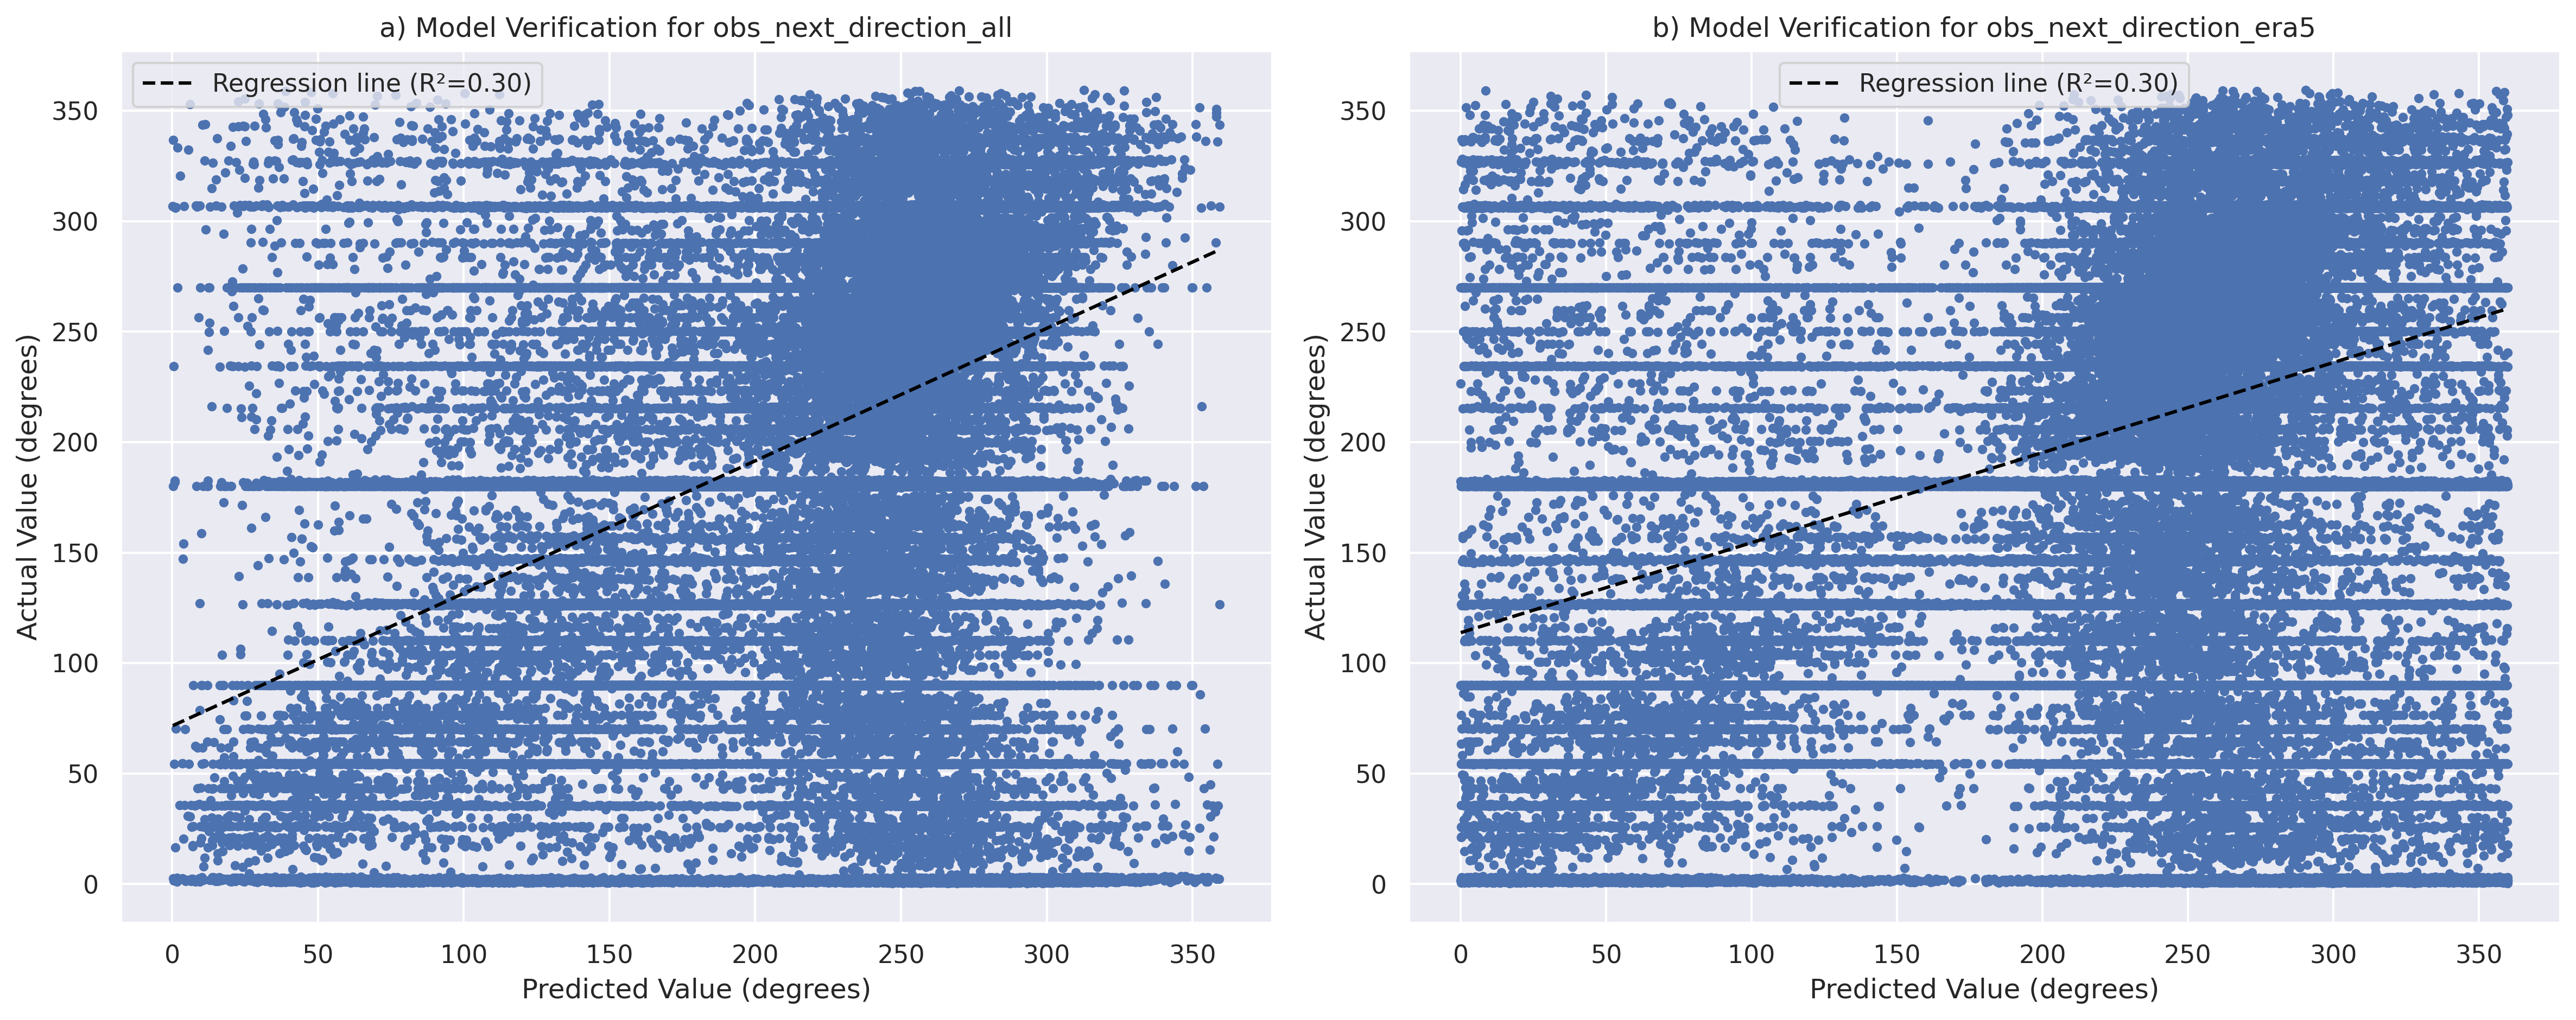
\includegraphics[width=\textwidth]{../figures/generated/experiments/obs_next_direction/obs_next_direction_summary.png}
    \caption{Comparison of performance and top features for next direction.}
    \label{fig:obs_direction_summary}
\end{figure}

\subsection{Next Distance}

\begin{figure}[ht]
    \centering
    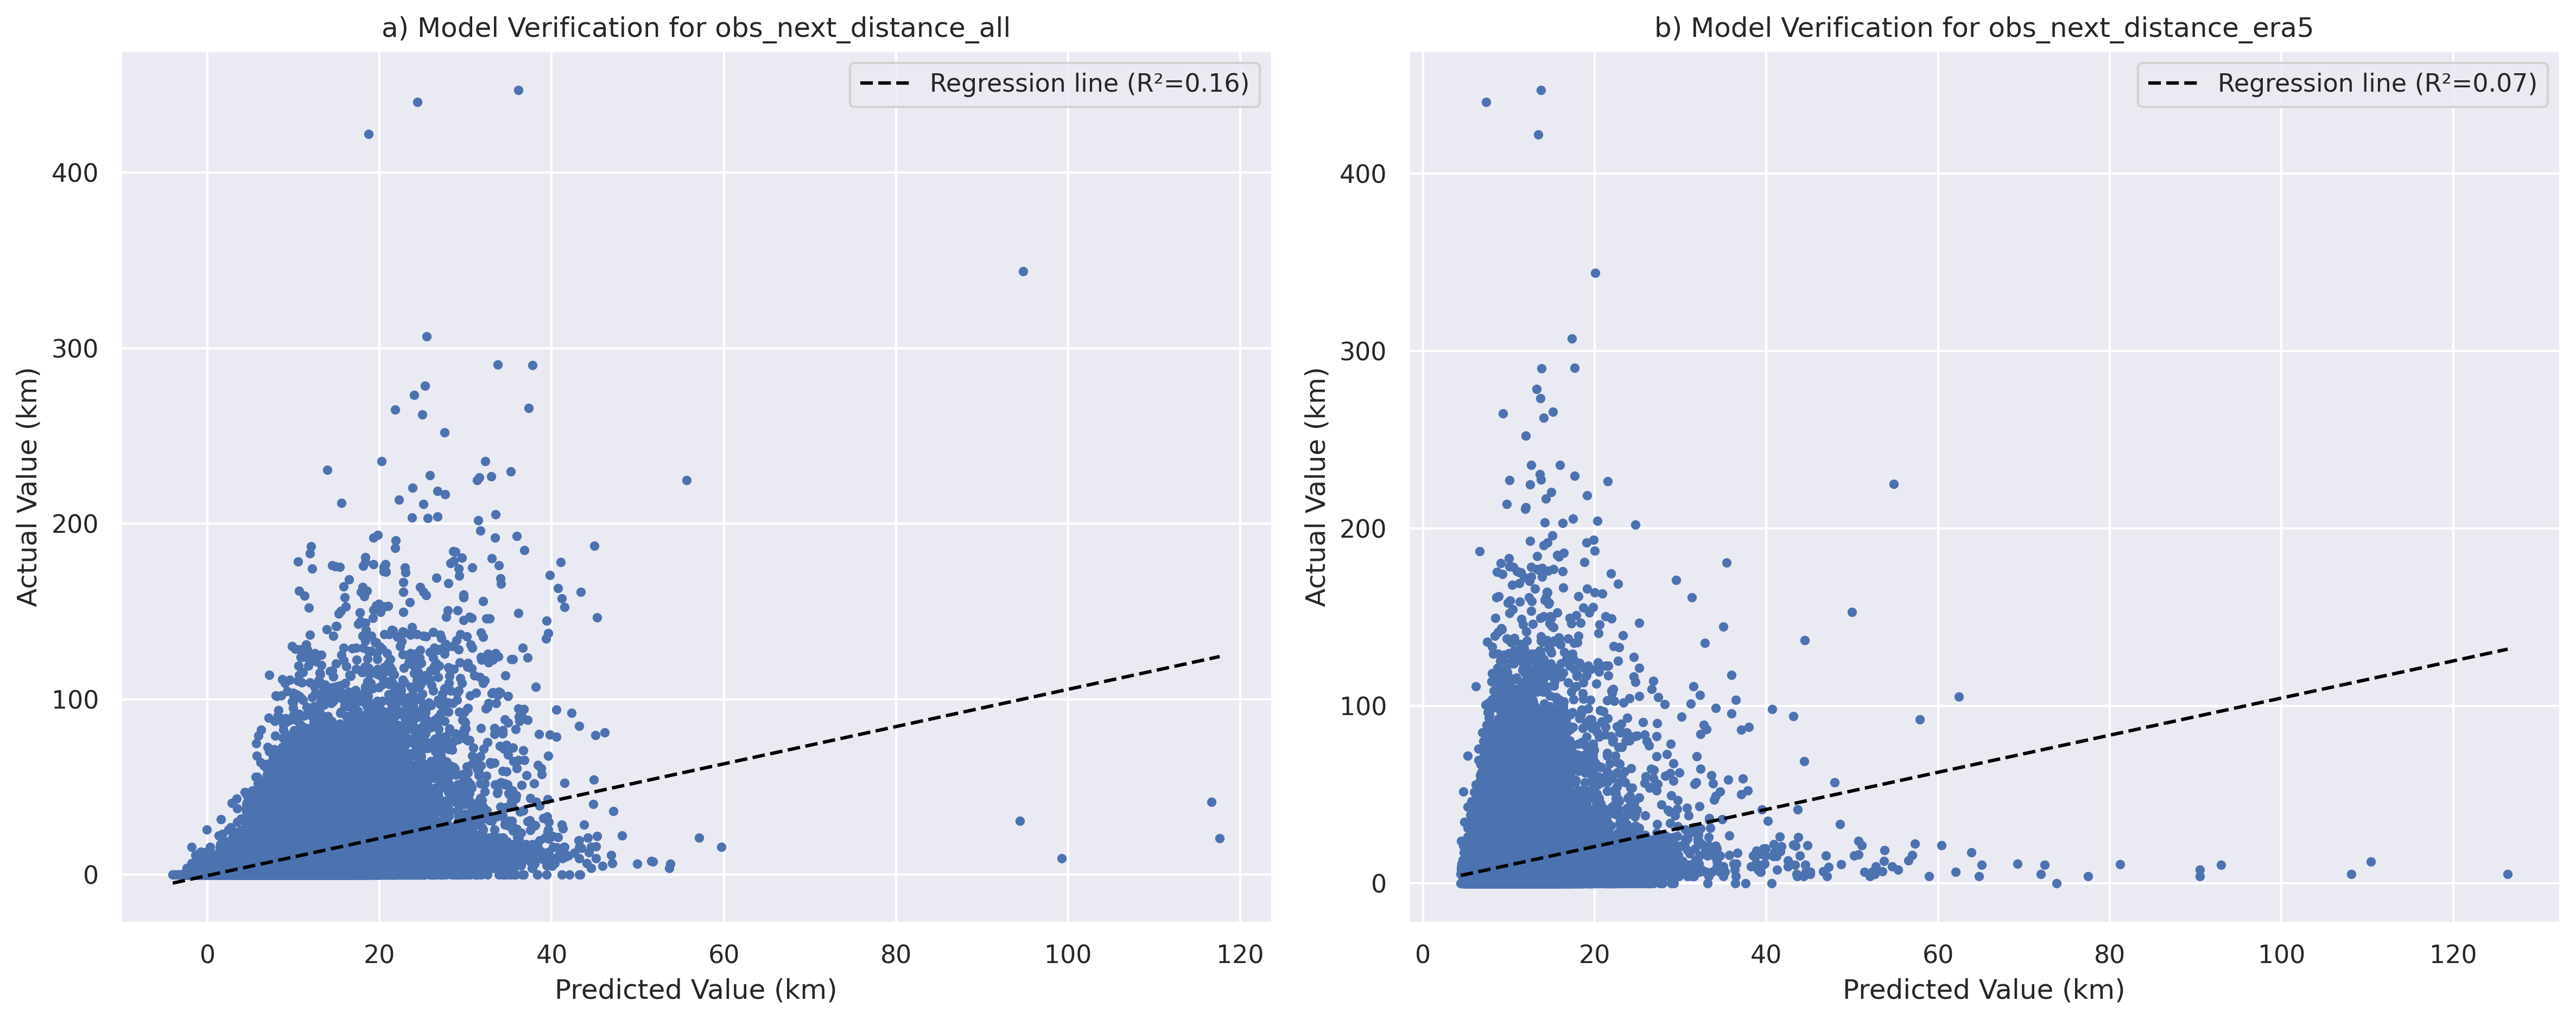
\includegraphics[width=\textwidth]{../figures/generated/experiments/obs_next_distance/obs_next_distance_summary.png}
    \caption{Comparison of performance and top features for next distance.}
    \label{fig:obs_distance_summary}
\end{figure}

\section{SHAP Correlation Heatmaps}
\label{appn:shap-heatmaps}

\subsection{Storm Maximum Intensity}
\label{appn:shap-heatmaps-smi}

\subsubsection{All Feature Set}
\begin{figure}[ht]
    \centering
    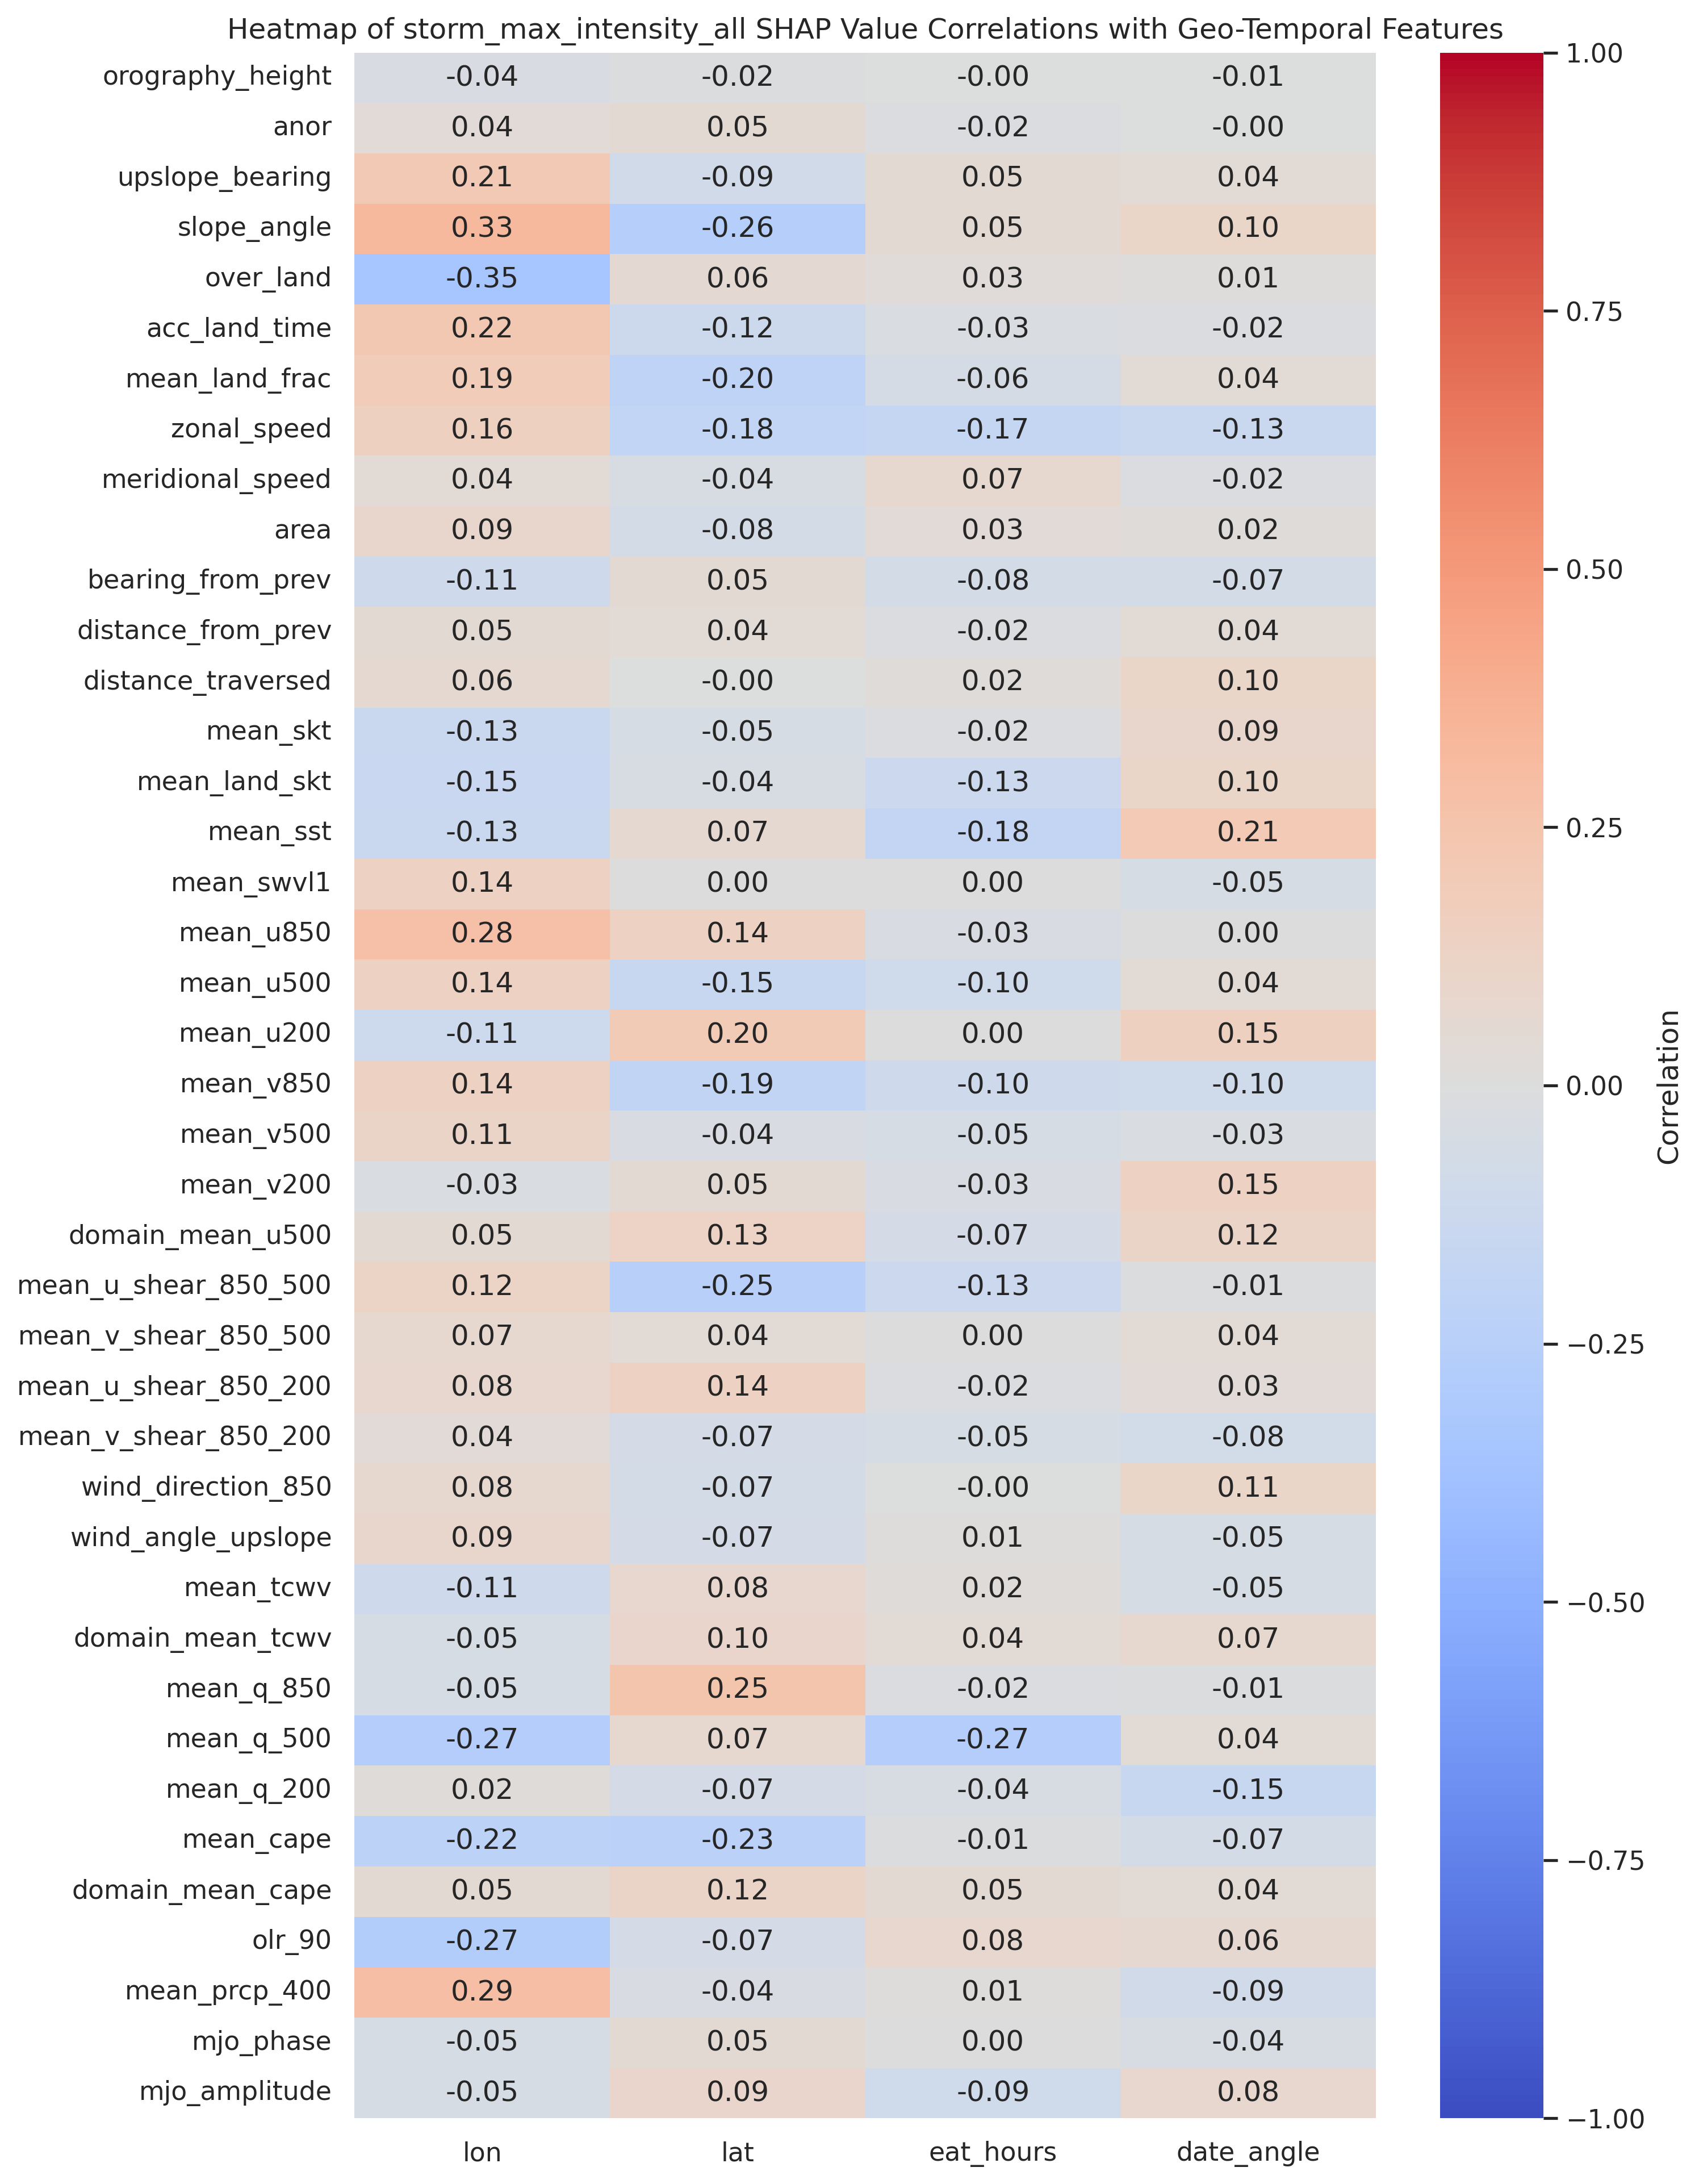
\includegraphics[width=\textwidth]{../figures/generated/experiments/storm_max_intensity/storm_max_intensity_all_shap_correlation_heatmap.png}
    \caption{Correlation heatmap of \acrshort{shap} values against latitude, longitude, time of day and time of year, for storm maximum intensity prediction task using all features.}
    \label{fig:storm_max_intensity_all_shap_heatmap}
\end{figure}

\subsubsection{ERA5 Feature Set}
\begin{figure}[ht]
    \centering
    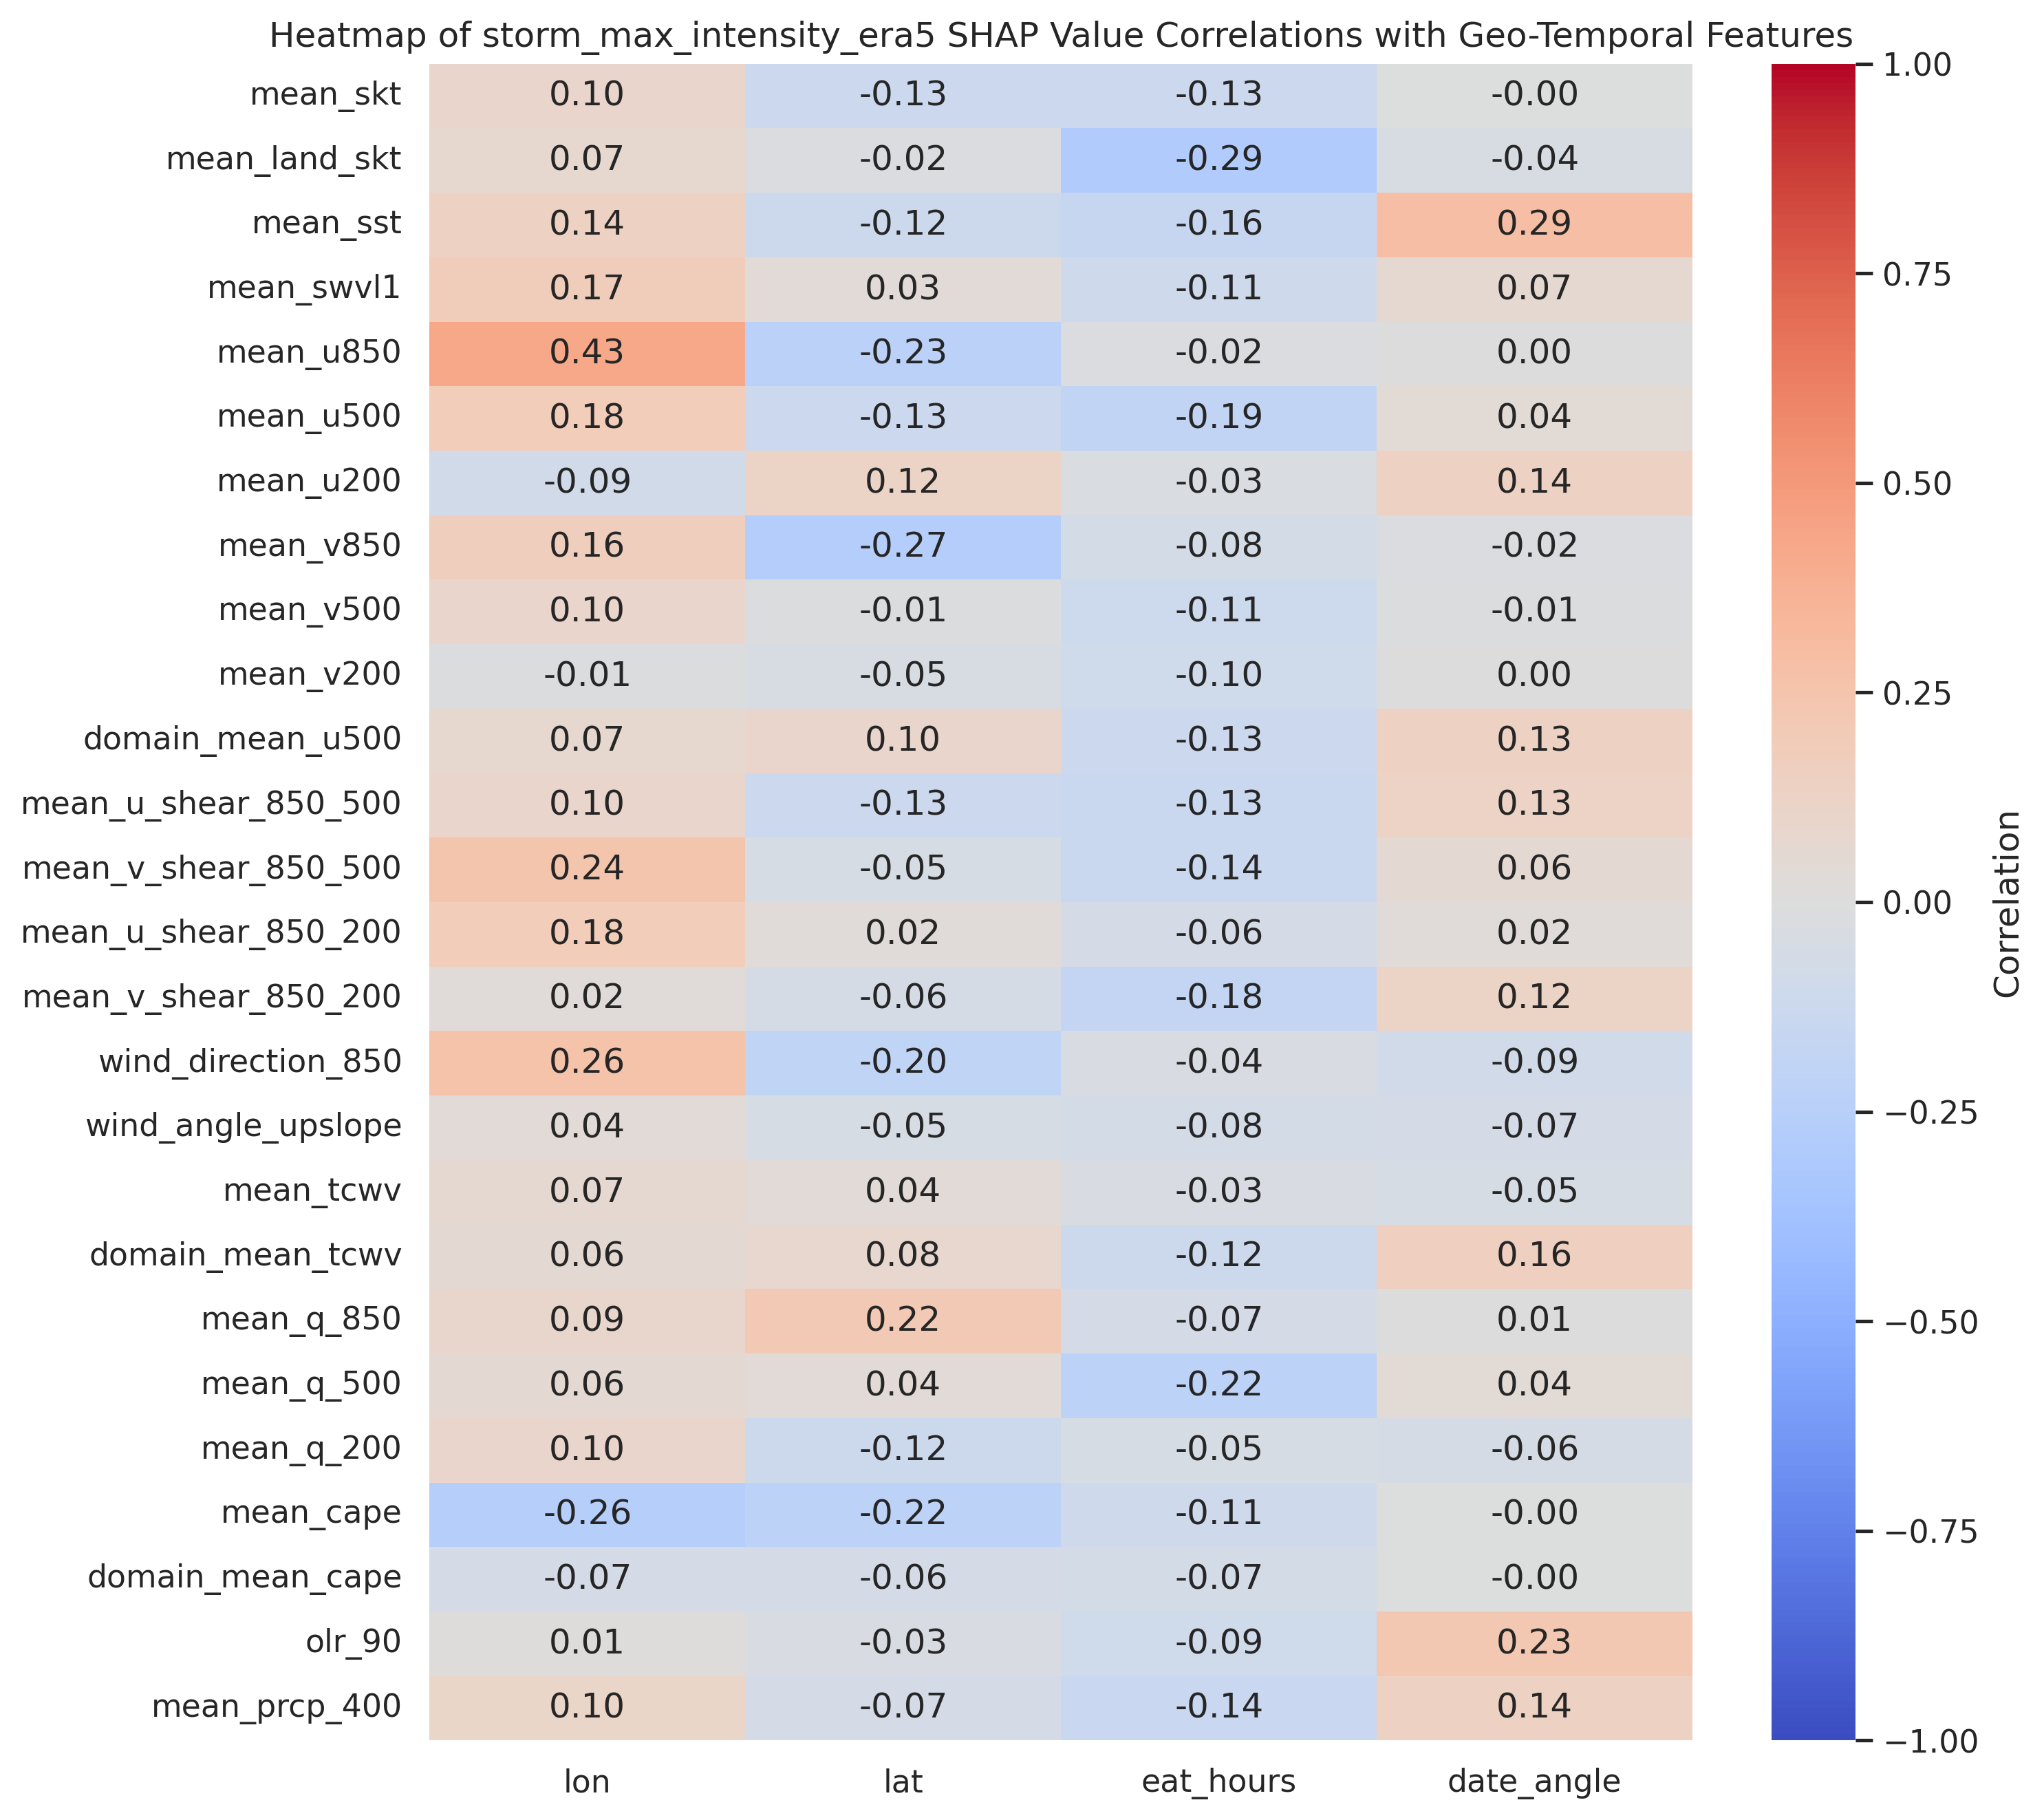
\includegraphics[width=\textwidth]{../figures/generated/experiments/storm_max_intensity/storm_max_intensity_era5_shap_correlation_heatmap.png}
    \caption{Correlation heatmap of \acrshort{shap} values against latitude, longitude, time of day and time of year, for storm maximum intensity prediction task using ERA5 features.}
    \label{fig:storm_max_intensity_era5_shap_heatmap}
\end{figure}

\subsection{Storm Direction}
\label{appn:shap-heatmaps-sd}

\subsubsection{All Feature Set}
\begin{figure}[ht]
    \centering
    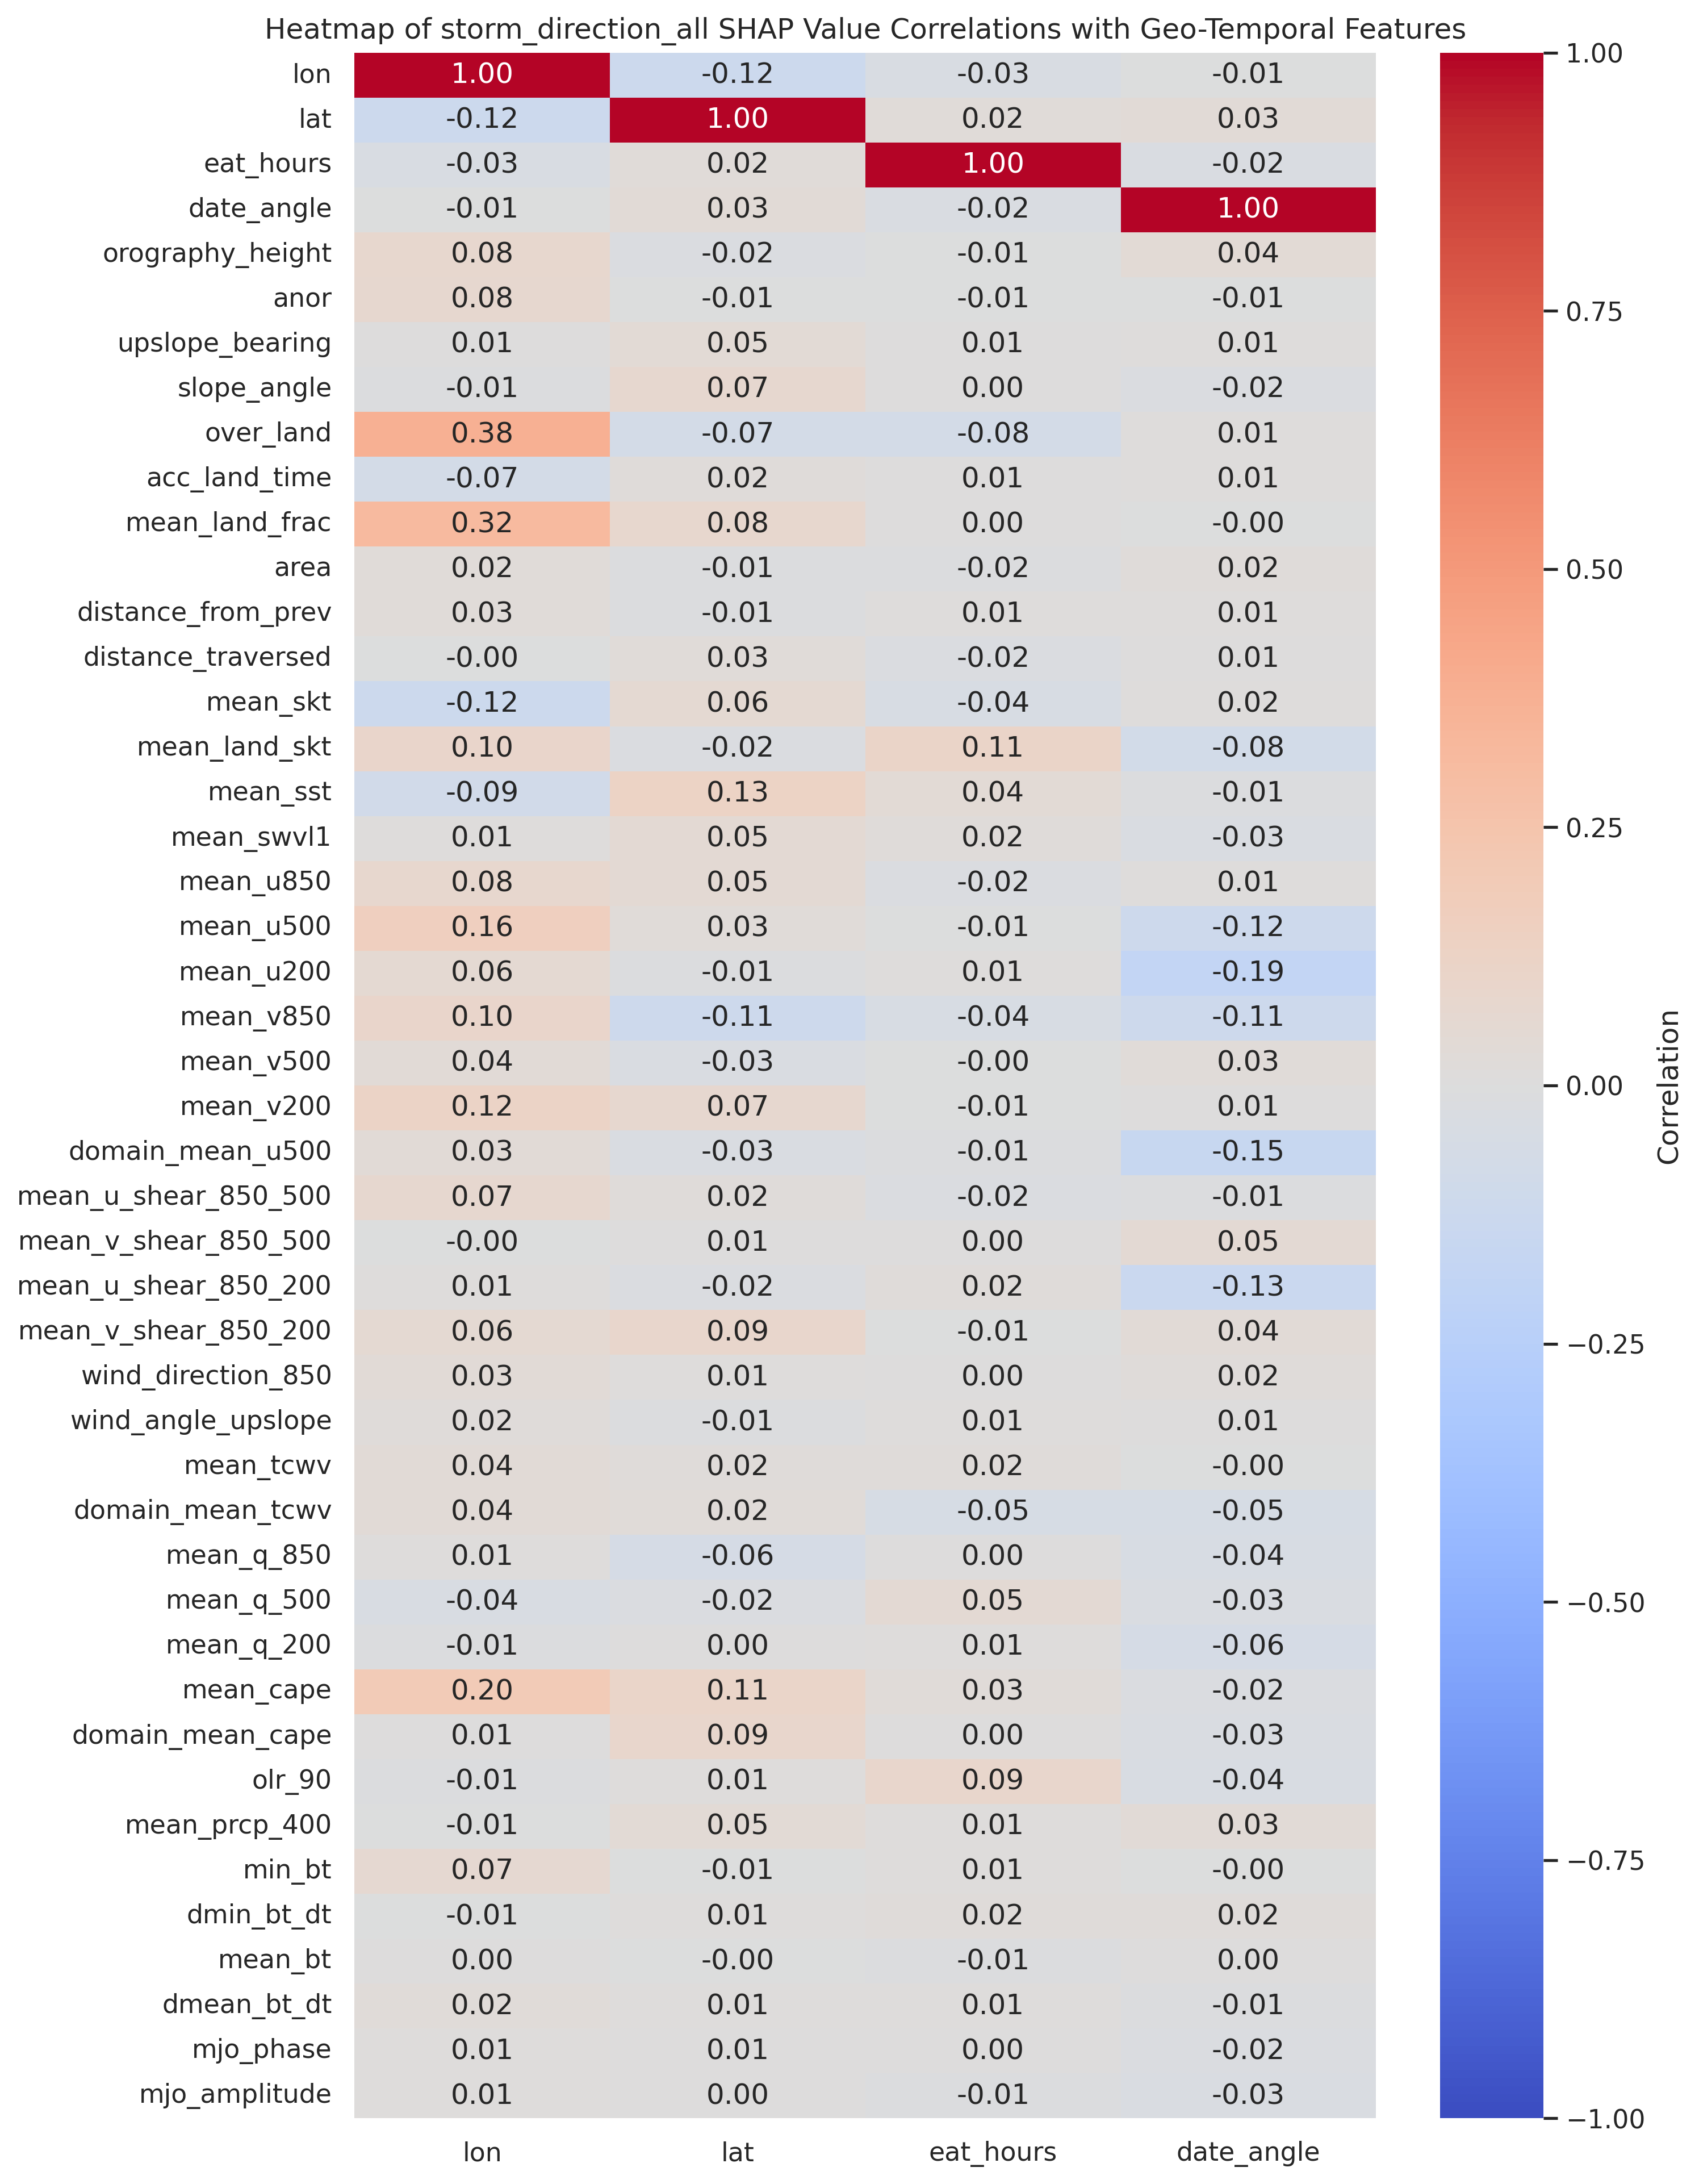
\includegraphics[width=\textwidth]{../figures/generated/experiments/storm_direction/storm_direction_all_shap_correlation_heatmap.png}
    \caption{Correlation heatmap of \acrshort{shap} values against latitude, longitude, time of day and time of year, for storm direction prediction task using all features.}
    \label{fig:storm_direction_all_shap_heatmap}
\end{figure}

\subsubsection{ERA5 Feature Set}
\begin{figure}[ht]
    \centering
    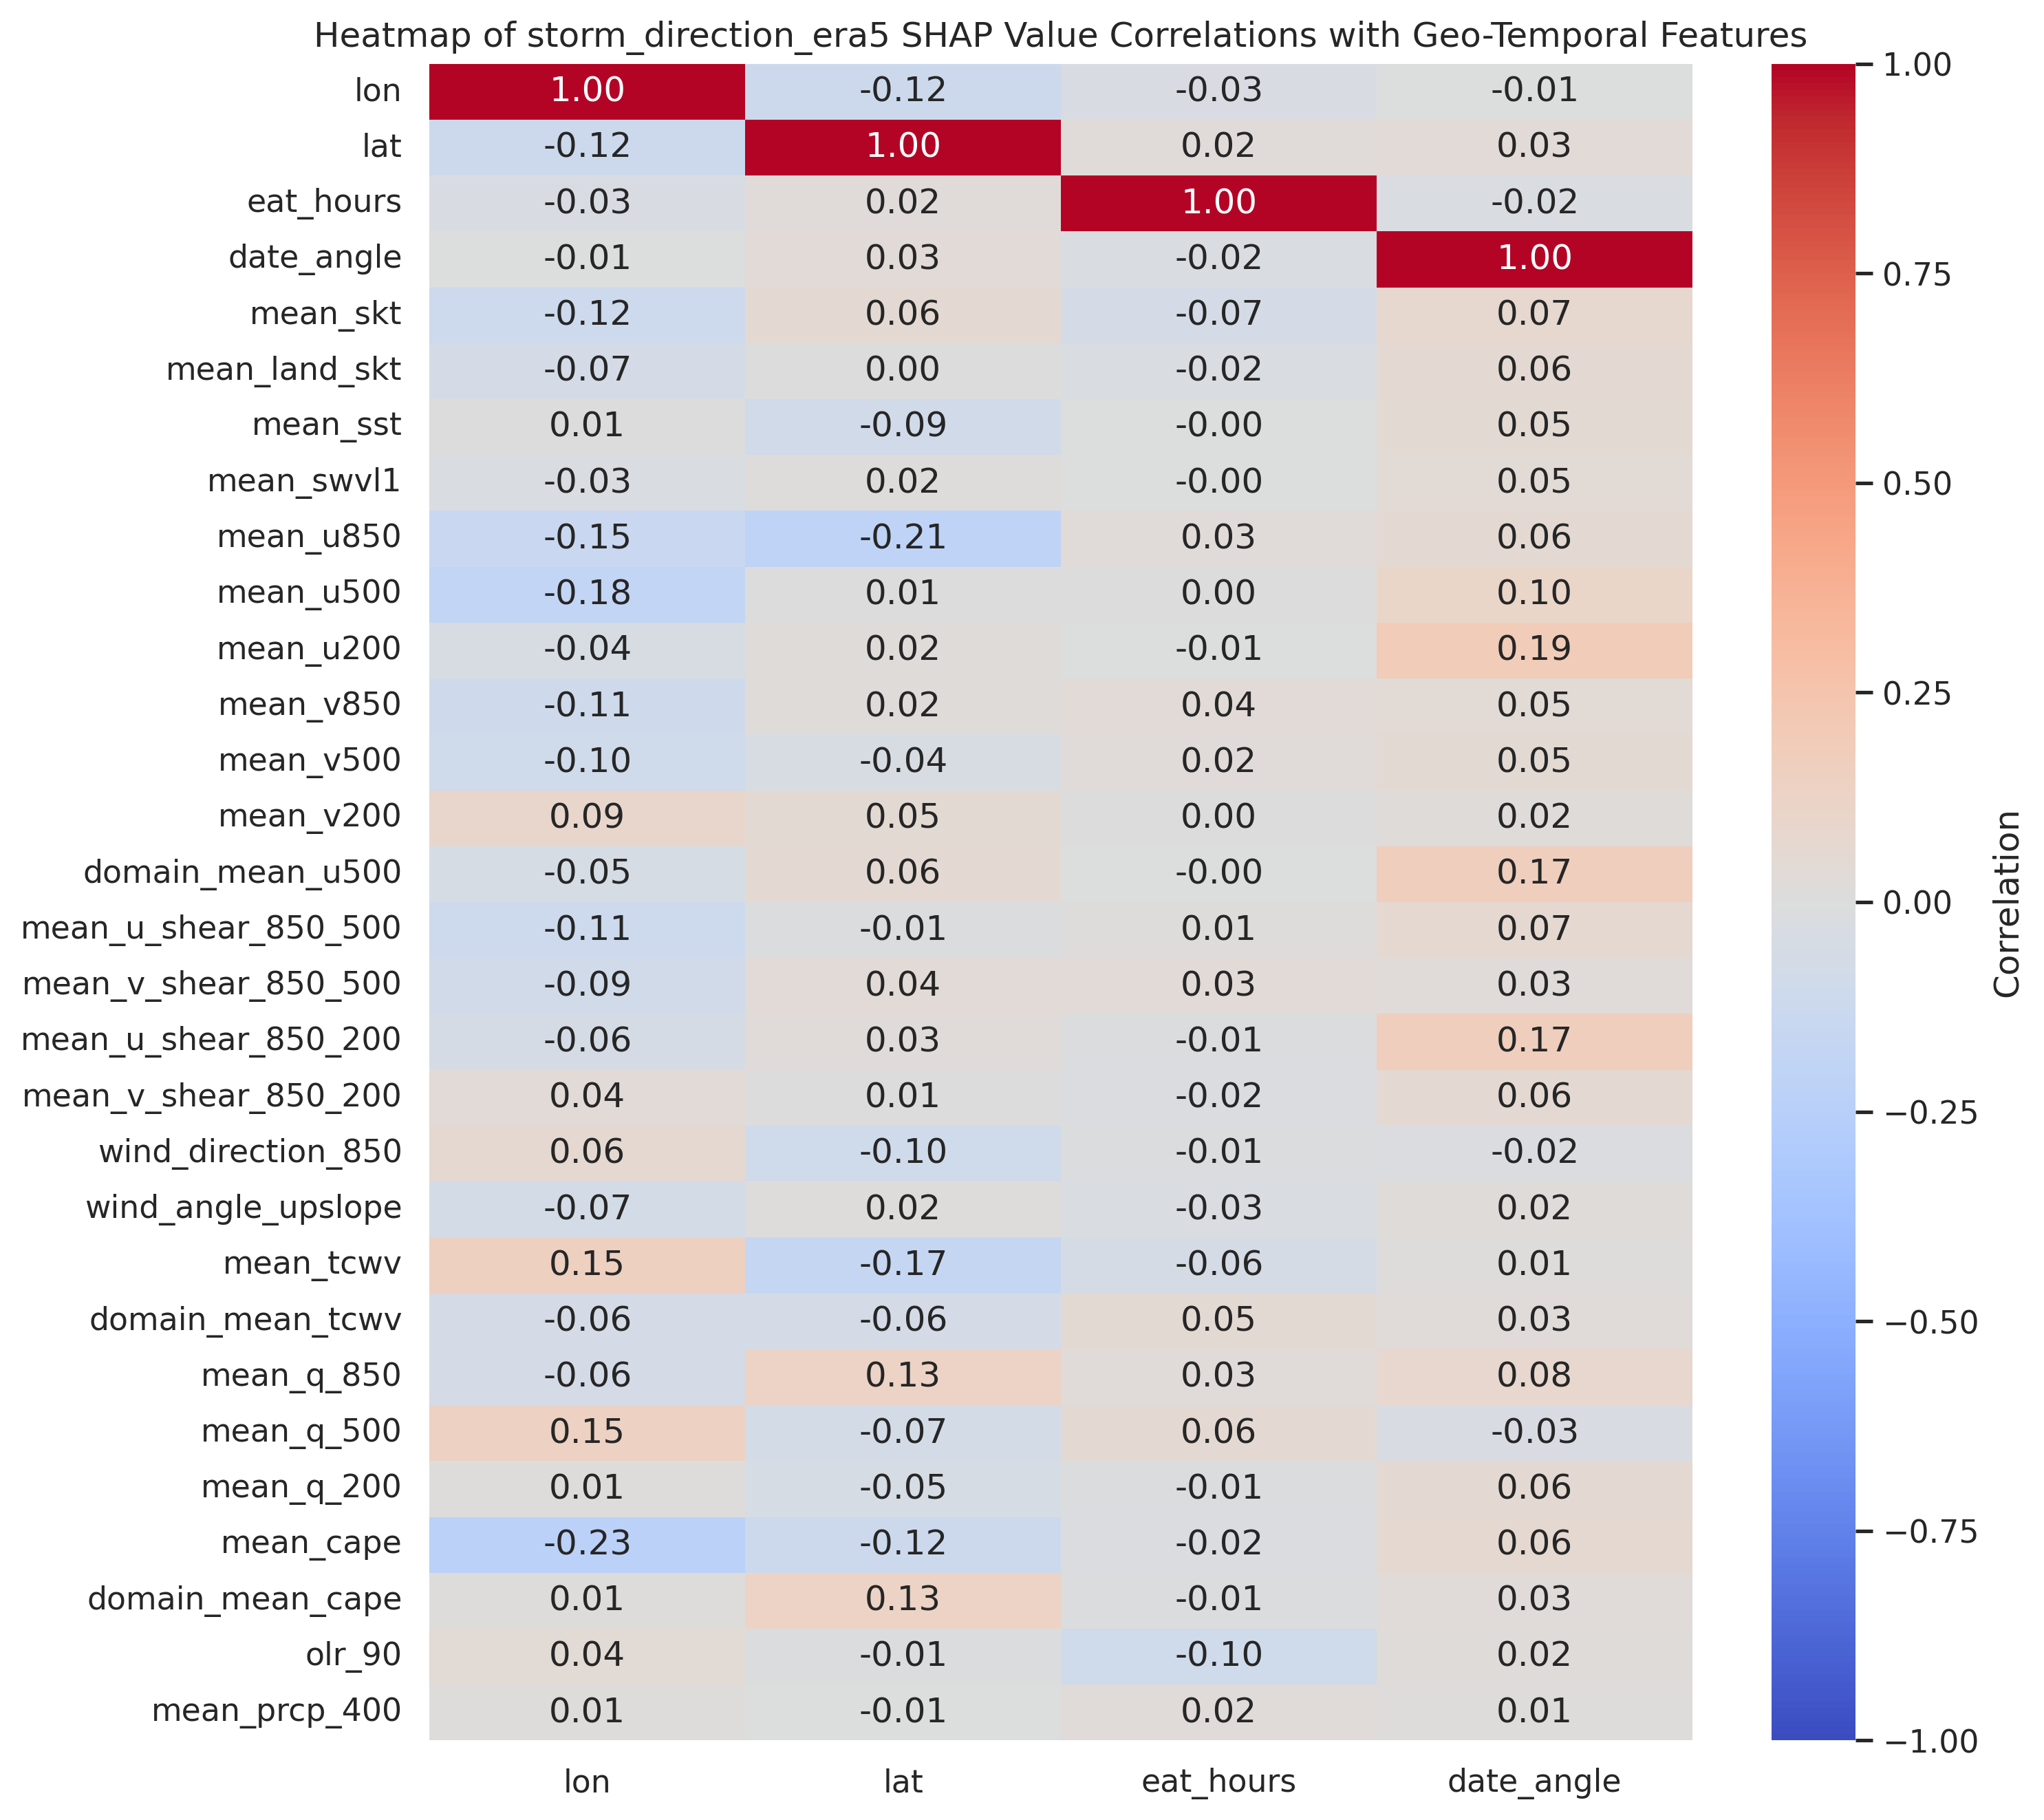
\includegraphics[width=\textwidth]{../figures/generated/experiments/storm_direction/storm_direction_era5_shap_correlation_heatmap.png}
    \caption{Correlation heatmap of \acrshort{shap} values against latitude, longitude, time of day and time of year, for storm direction prediction task using ERA5 features.}
    \label{fig:storm_direction_era5_shap_heatmap}
\end{figure}

\subsection{Intensification}
\label{appn:shap-heatmaps-int}

\subsubsection{All Feature Set}
\begin{figure}[ht]
    \centering
    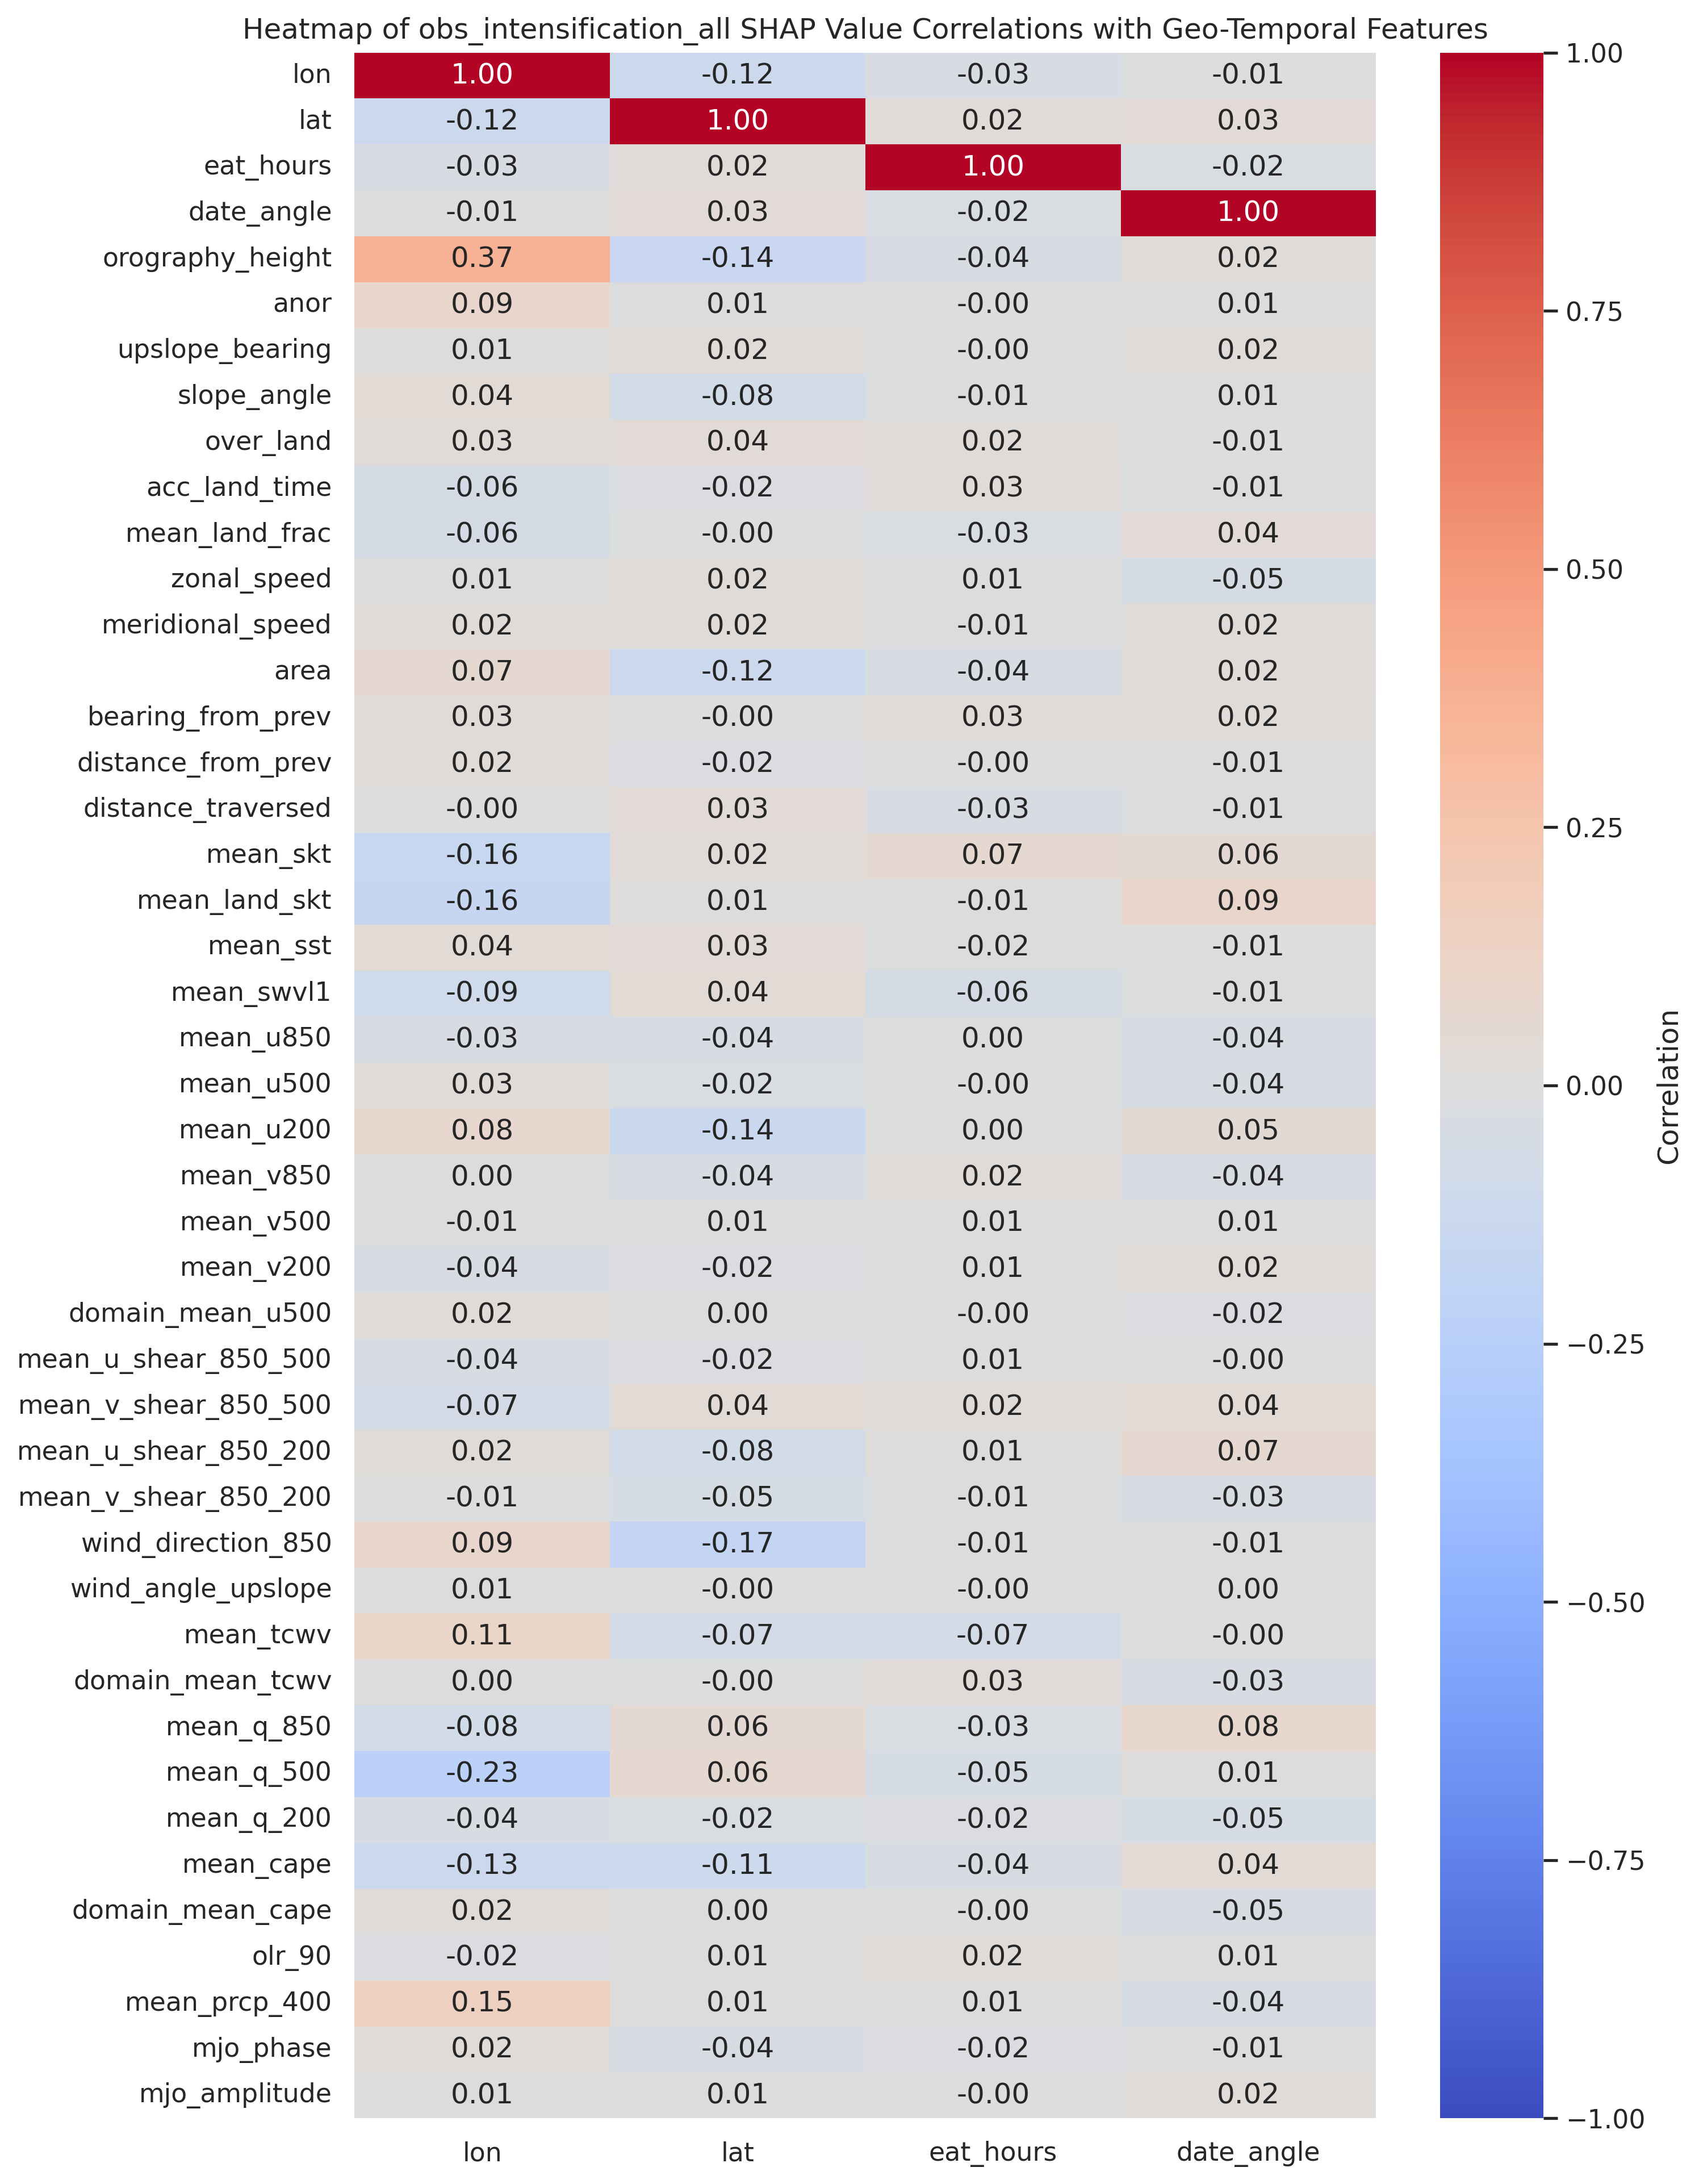
\includegraphics[width=\textwidth]{../figures/generated/experiments/obs_intensification/obs_intensification_all_shap_correlation_heatmap.png}
    \caption{Correlation heatmap of \acrshort{shap} values against latitude, longitude, time of day and time of year, for intensification prediction task using all features.}
    \label{fig:obs_intensification_all_shap_heatmap}
\end{figure}

\subsubsection{ERA5 Feature Set}
\begin{figure}[ht]
    \centering
    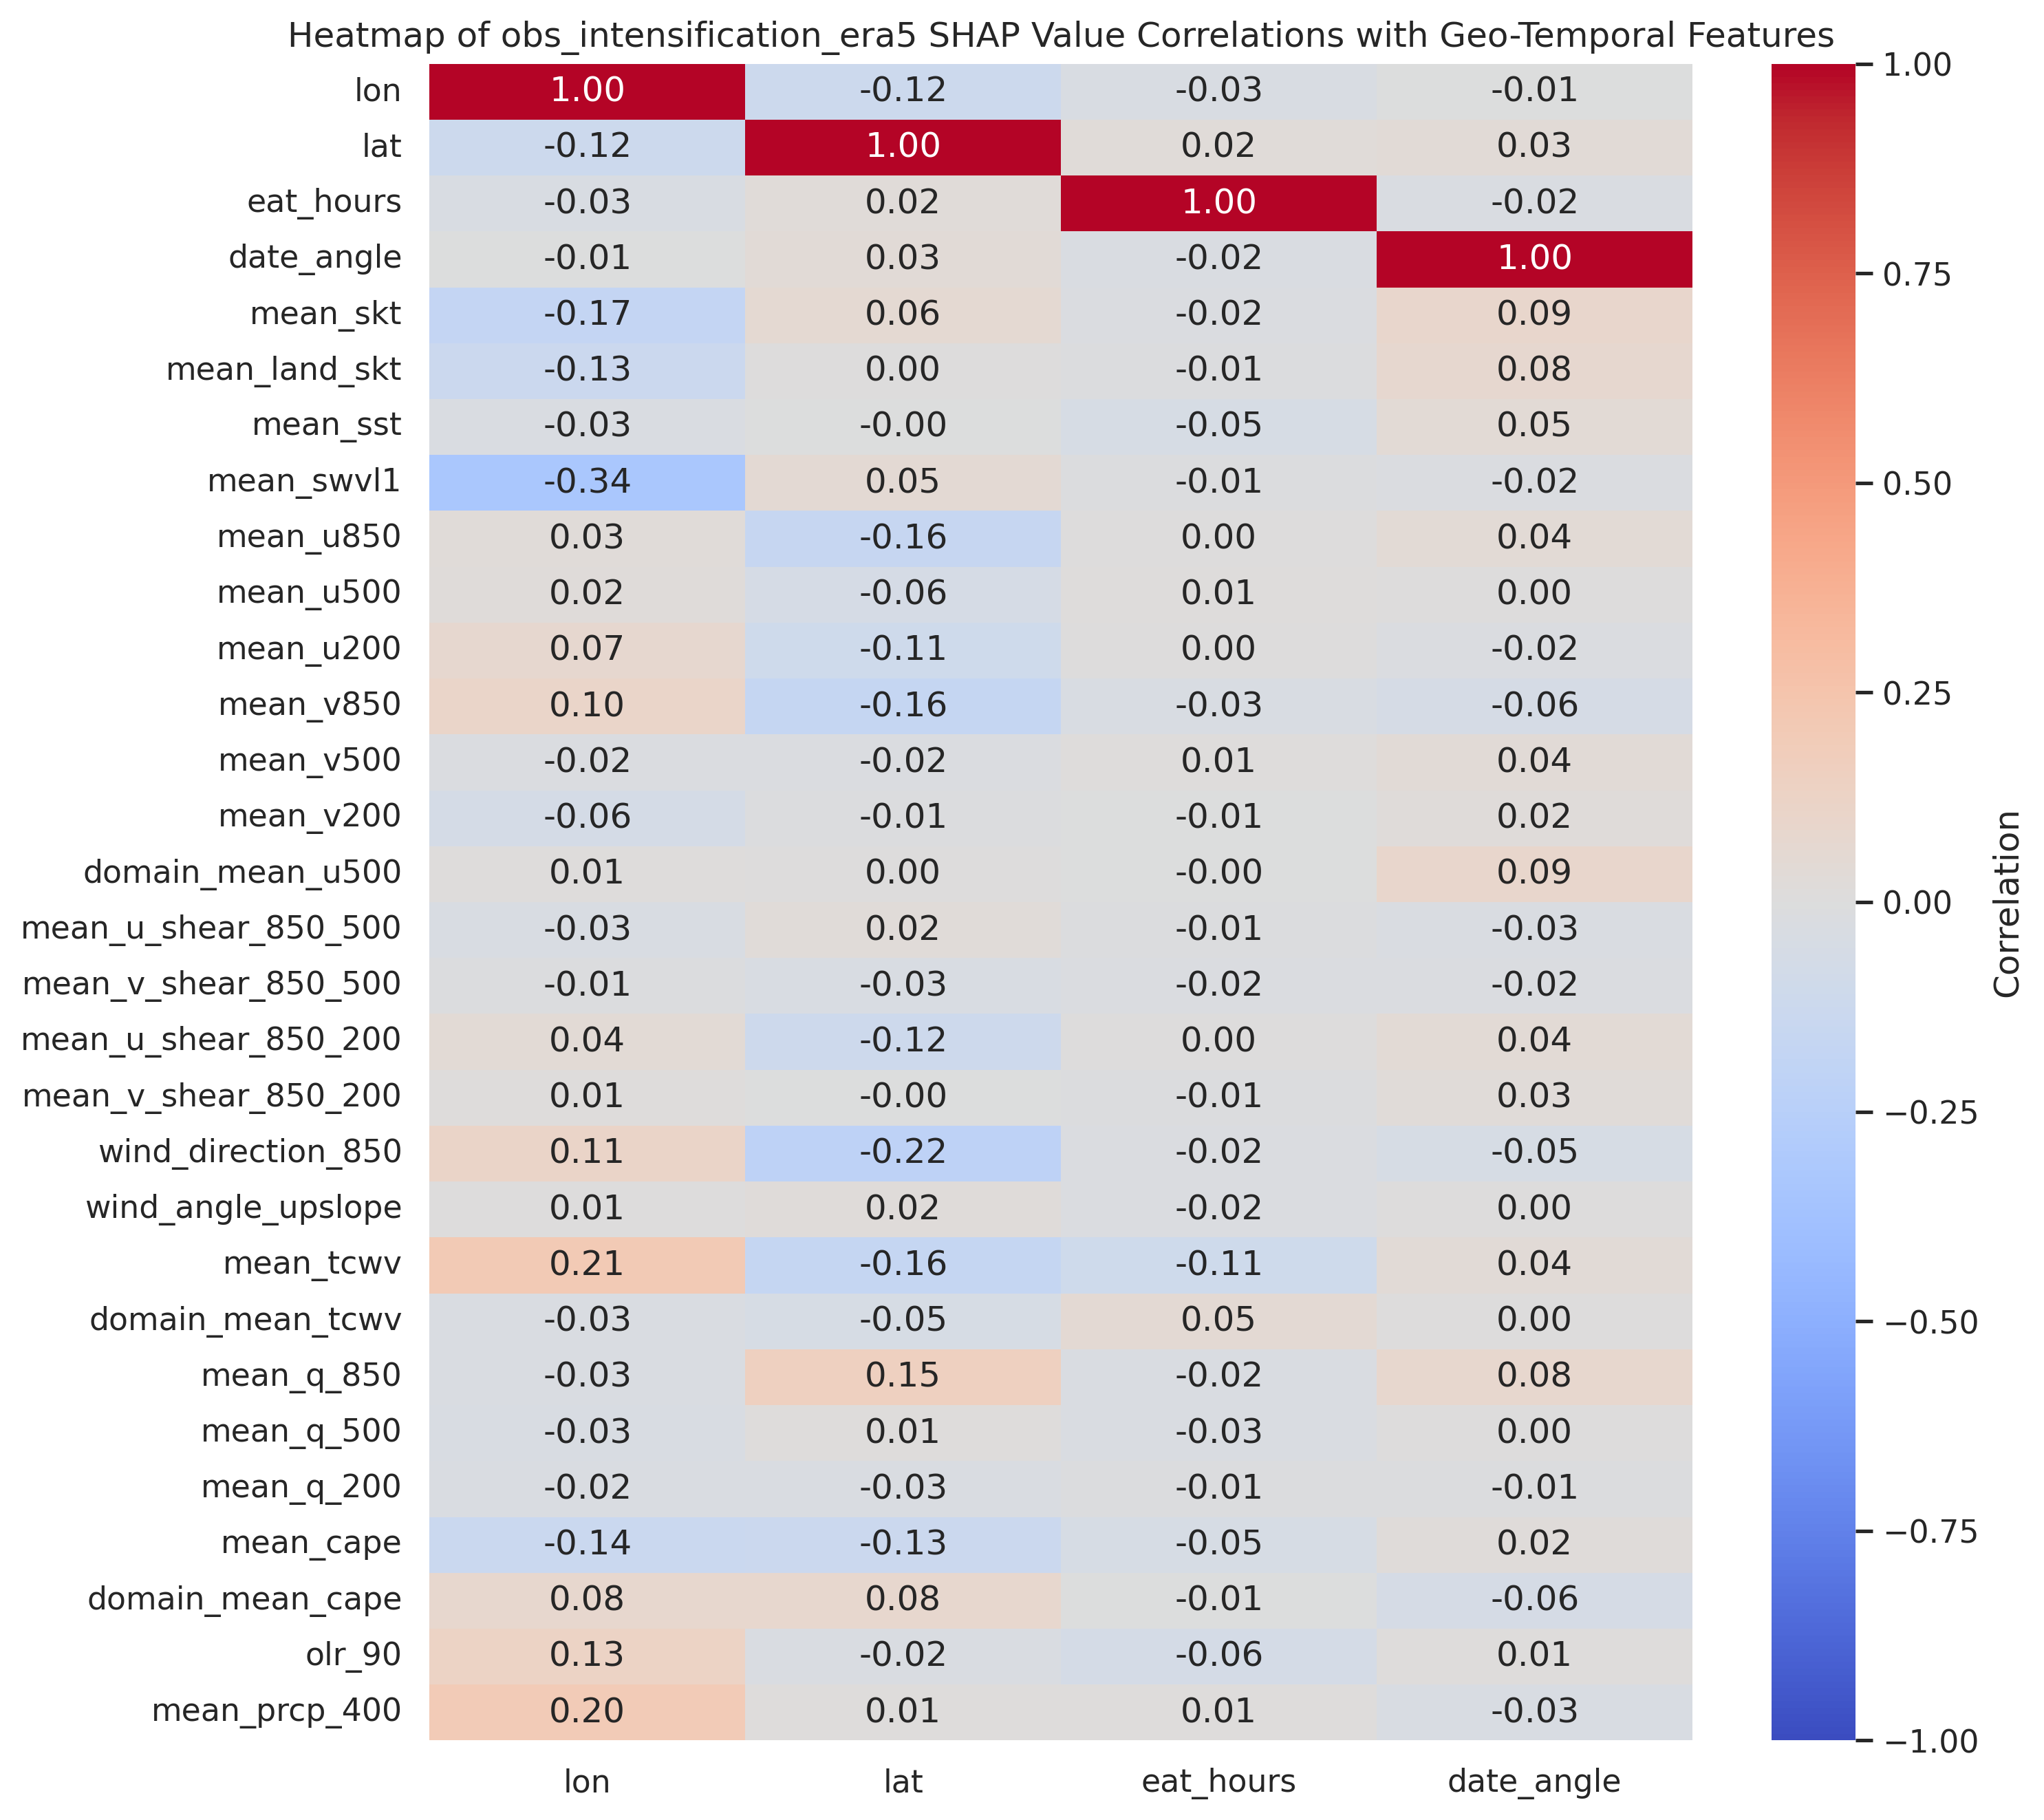
\includegraphics[width=\textwidth]{../figures/generated/experiments/obs_intensification/obs_intensification_era5_shap_correlation_heatmap.png}
    \caption{Correlation heatmap of \acrshort{shap} values against latitude, longitude, time of day and time of year, for intensification prediction task using ERA5 features.}
    \label{fig:obs_intensification_era5_shap_heatmap}
\end{figure}

\subsection{Precipitation}
\label{appn:shap-heatmaps-precip}

\subsubsection{All Feature Set}
\begin{figure}[ht]
    \centering
    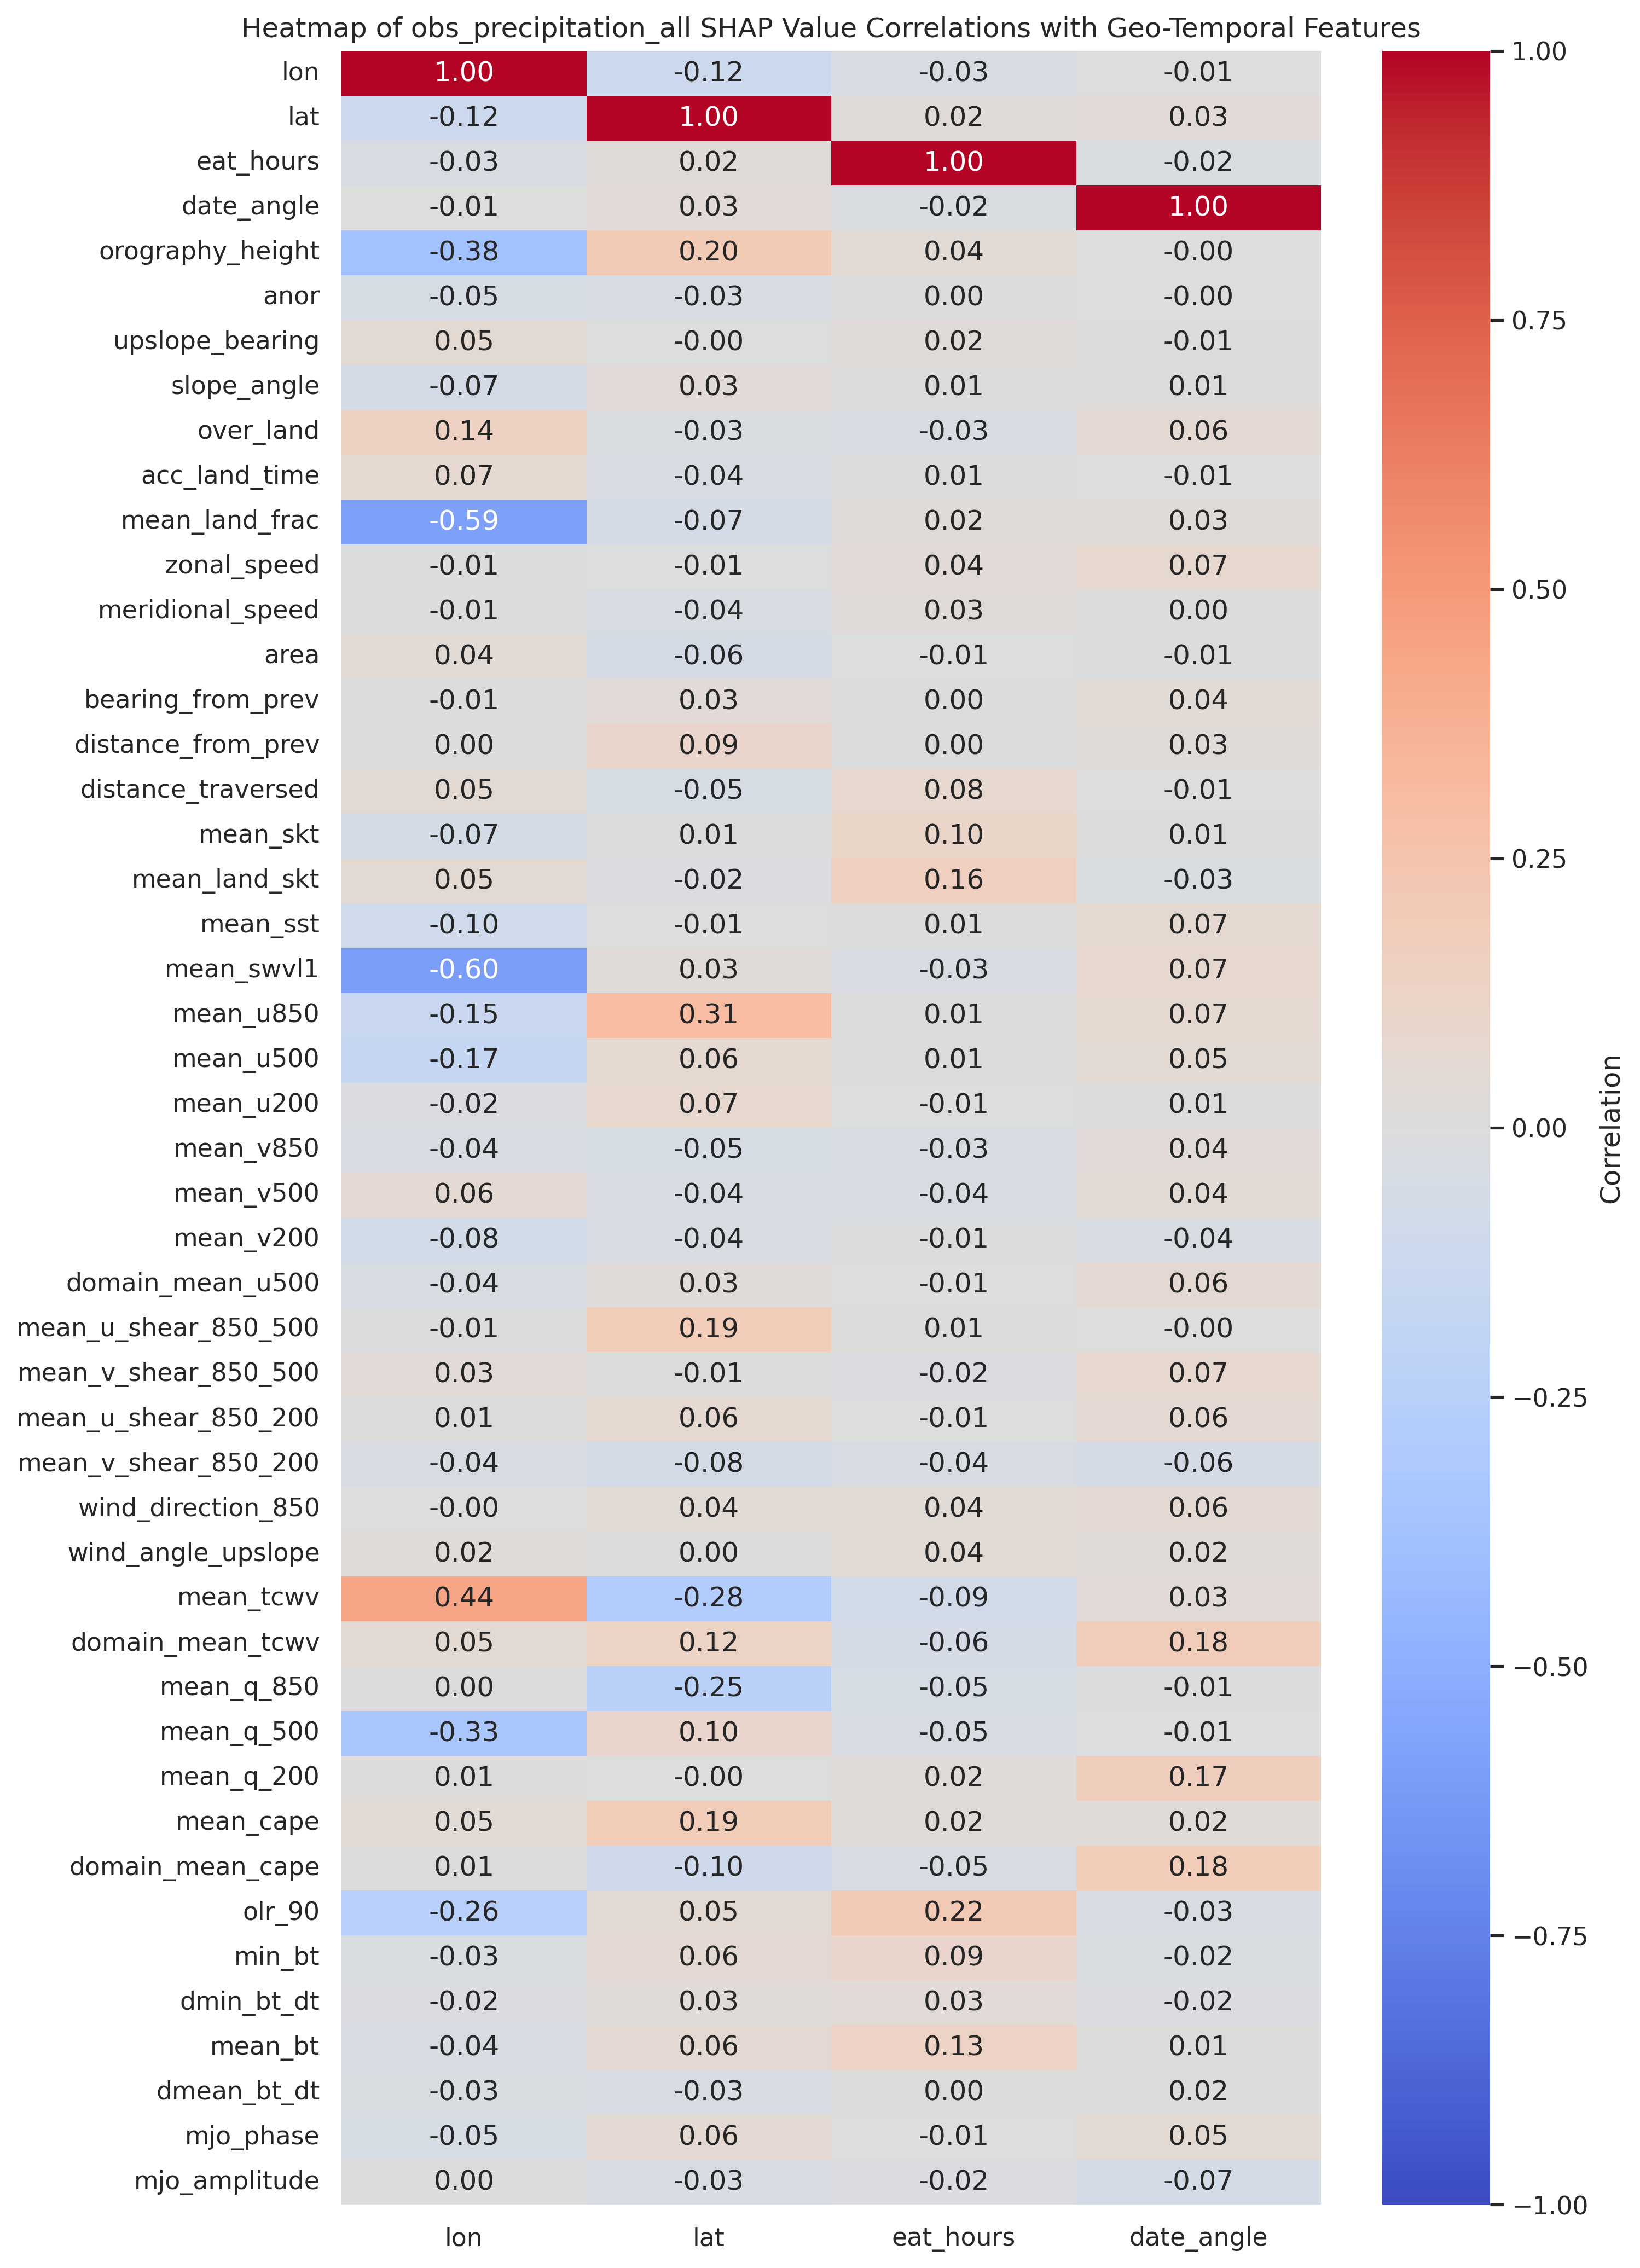
\includegraphics[width=\textwidth]{../figures/generated/experiments/obs_precipitation/obs_precipitation_all_shap_correlation_heatmap.png}
    \caption{Correlation heatmap of \acrshort{shap} values against latitude, longitude, time of day and time of year, for storm precipitation prediction task using all features.}
    \label{fig:obs_precipitation_all_shap_heatmap}
\end{figure}

\subsubsection{ERA5 Feature Set}
\begin{figure}[ht]
    \centering
    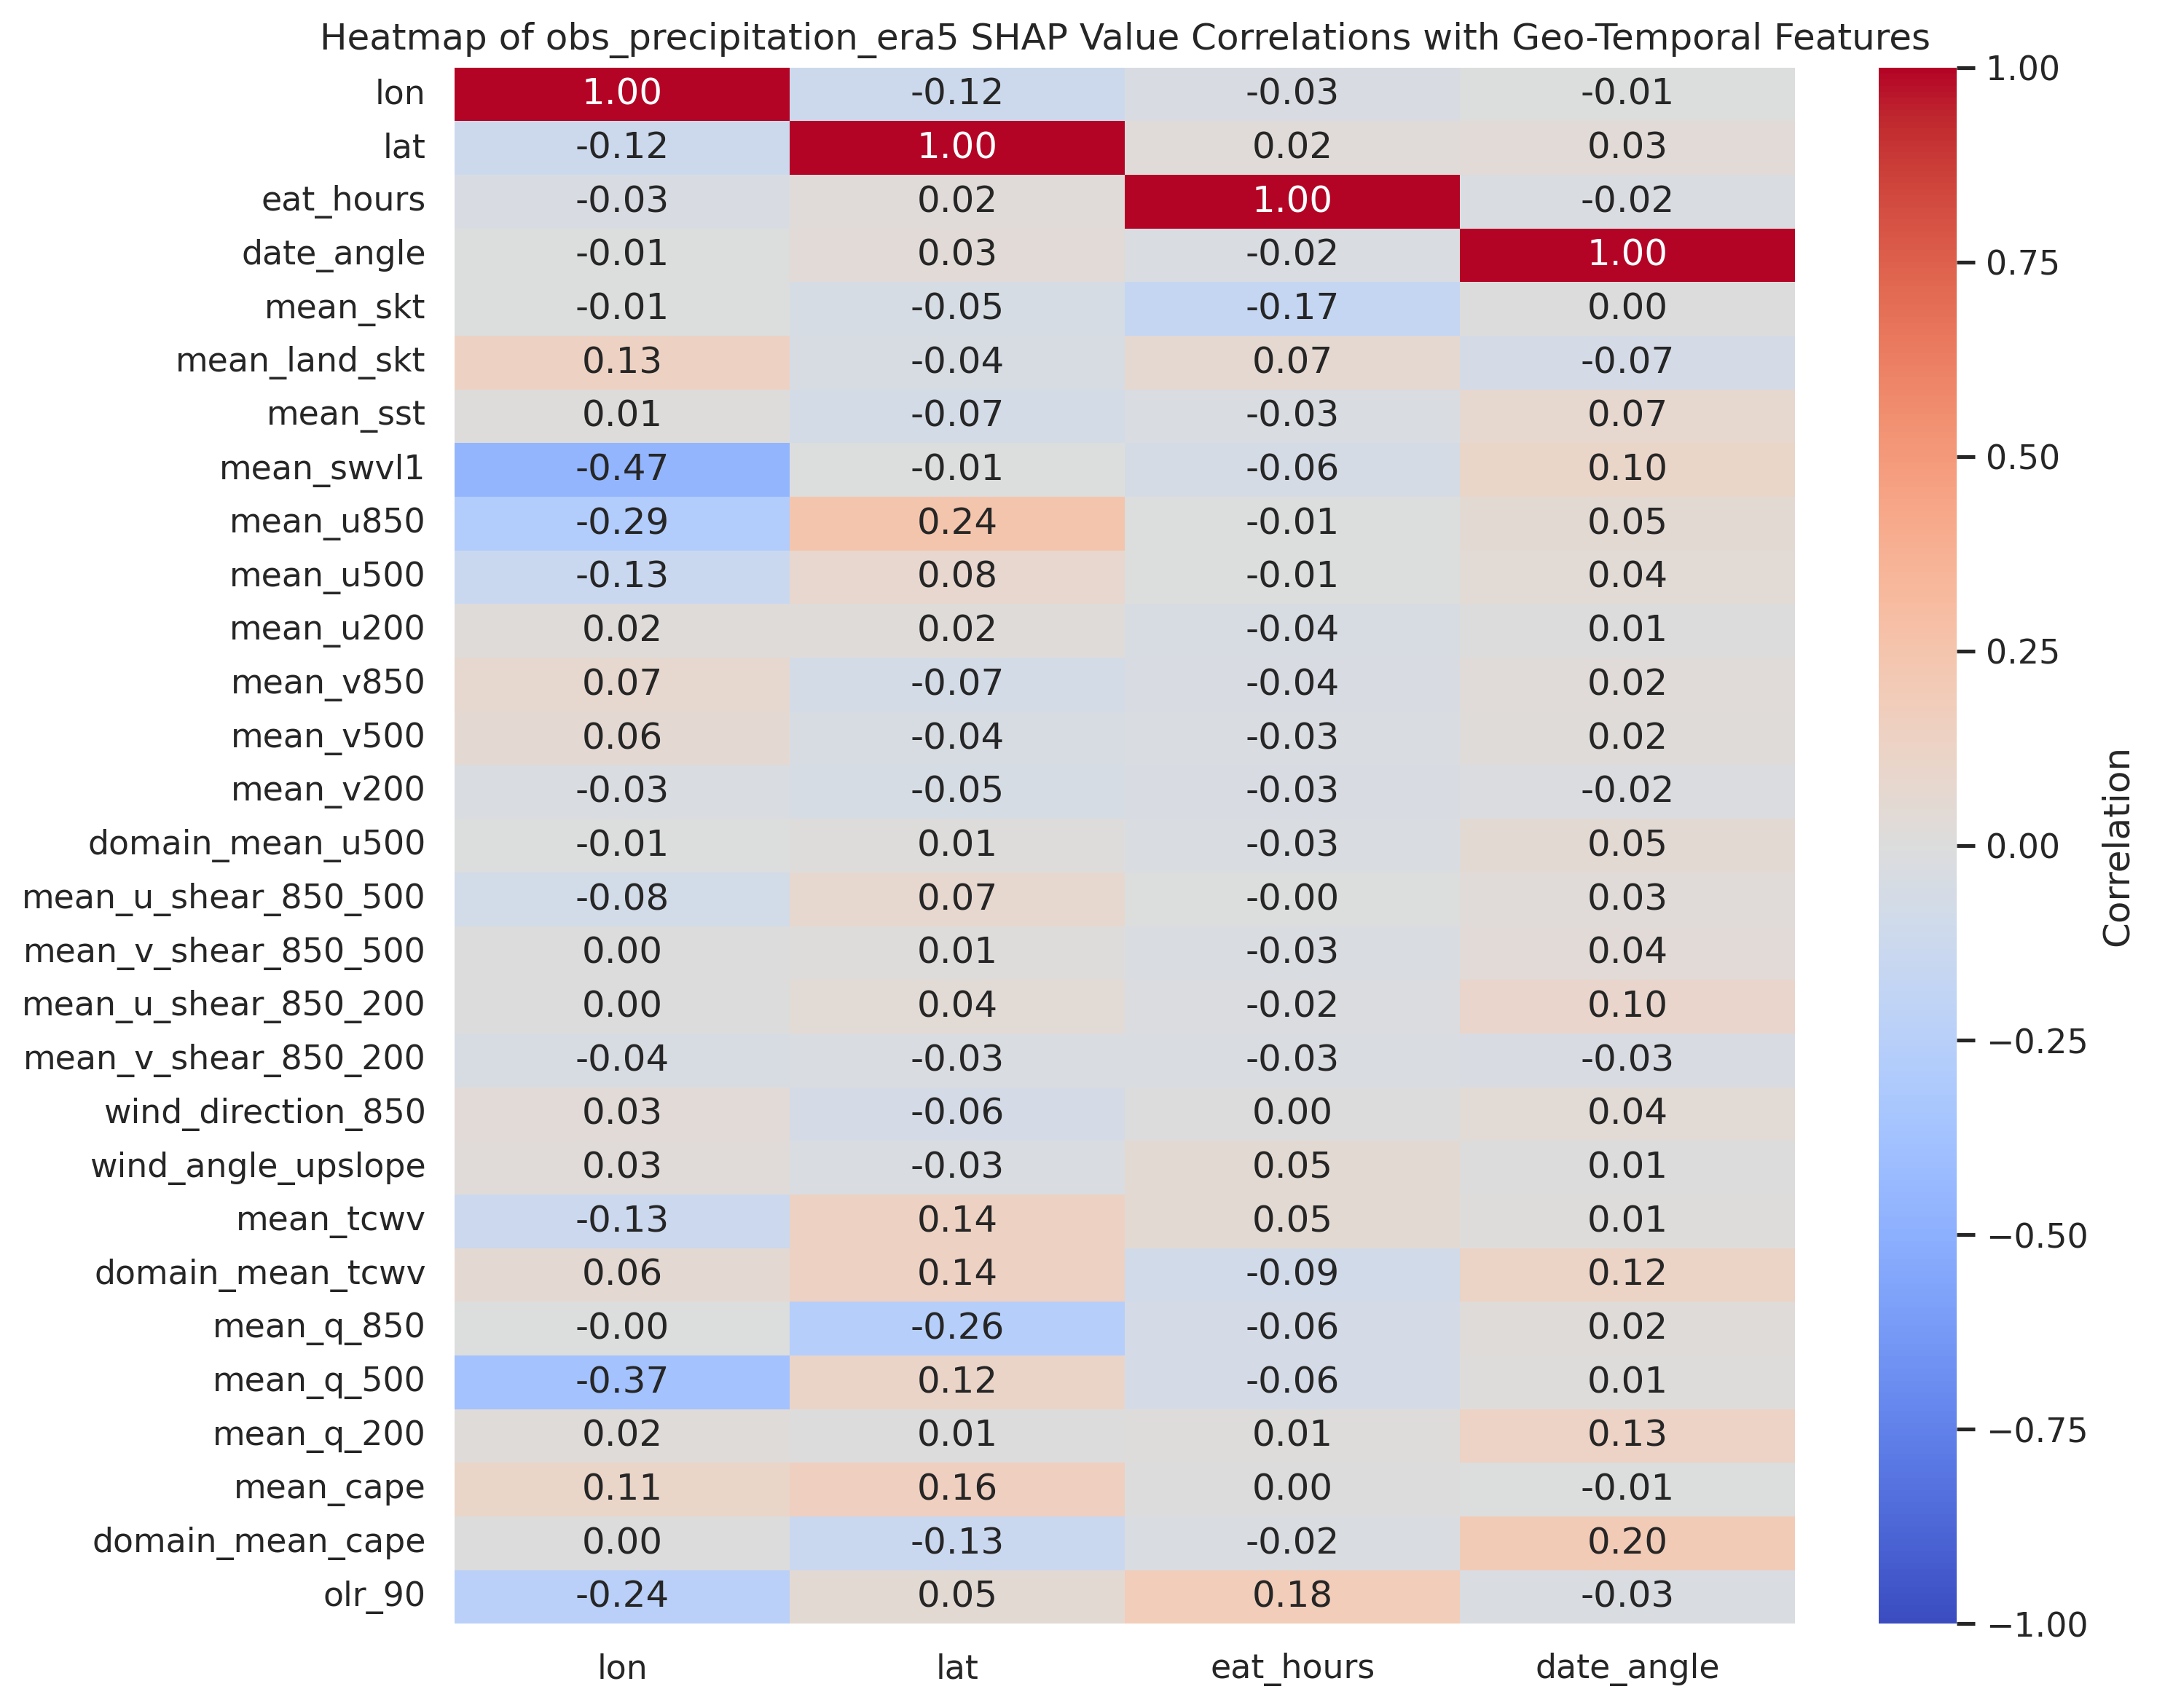
\includegraphics[width=\textwidth]{../figures/generated/experiments/obs_precipitation/obs_precipitation_era5_shap_correlation_heatmap.png}
    \caption{Correlation heatmap of \acrshort{shap} values against latitude, longitude, time of day and time of year, for storm precipitation prediction task using ERA5 features.}
    \label{fig:obs_precipitation_era5_shap_heatmap}
\end{figure}